% ******************************* PhD Thesis Template **************************
% Please have a look at the README.md file for info on how to use the template

\documentclass[a4paper,12pt,times,numbered,print,index]{Classes/PhDThesisPSnPDF}

% ******************************************************************************
% ******************************* Class Options ********************************
% *********************** See README for more details **************************
% ******************************************************************************

% `a4paper'(The University of Cambridge PhD thesis guidelines recommends a page
% size a4 - default option) or `a5paper': A5 Paper size is also allowed as per
% the Cambridge University Engineering Deparment guidelines for PhD thesis
%
% `11pt' or `12pt'(default): Font Size 10pt is NOT recommended by the University
% guidelines
%
% `oneside' or `twoside'(default): Printing double side (twoside) or single
% side.
%
% `print': Use `print' for print version with appropriate margins and page
% layout. Leaving the options field blank will activate Online version.
%
% `index': For index at the end of the thesis
%
% `draftclassic': For draft mode without loading any images (same as draft in book)
%
% `draft': Special draft mode with line numbers, images, and water mark with
% timestamp and custom text. Position of the text can also be modified.
%
% `abstract': To generate only the title page and abstract page with
% dissertation title and name, to submit to the Student Registry
%
% `chapter`: This option enables only the specified chapter and it's references
%  Useful for review and corrections.
%
% ************************* Custom Page Margins ********************************
%
% `custommargin`: Use `custommargin' in options to activate custom page margins,
% which can be defined in the preamble.tex. Custom margin will override
% print/online margin setup.
%
% *********************** Choosing the Fonts in Class Options ******************
%
% `times' : Times font with math support. (The Cambridge University guidelines
% recommend using times)
%
% `fourier': Utopia Font with Fourier Math font (Font has to be installed)
%            It's a free font.
%
% `customfont': Use `customfont' option in the document class and load the
% package in the preamble.tex
%
% default or leave empty: `Latin Modern' font will be loaded.
%
% ********************** Choosing the Bibliography style ***********************
%
% `authoryear': For author-year citation eg., Krishna (2013)
%
% `numbered': (Default Option) For numbered and sorted citation e.g., [1,5,2]
%
% `custombib': Define your own bibliography style in the `preamble.tex' file.
%              `\RequirePackage[square, sort, numbers, authoryear]{natbib}'.
%              This can be also used to load biblatex instead of natbib
%              (See Preamble)
%
% **************************** Choosing the Page Style *************************
%
% `default (leave empty)': For Page Numbers in Header (Left Even, Right Odd) and
% Chapter Name in Header (Right Even) and Section Name (Left Odd). Blank Footer.
%
% `PageStyleI': Chapter Name next & Page Number on Even Side (Left Even).
% Section Name & Page Number in Header on Odd Side (Right Odd). Footer is empty.
%
% `PageStyleII': Chapter Name on Even Side (Left Even) in Header. Section Number
% and Section Name in Header on Odd Side (Right Odd). Page numbering in footer

% Uncomment to change page style
%\pagestyle{PageStyleII}

% ********************************** Preamble **********************************
% Preamble: Contains packages and user-defined commands and settings
%TC:ignore
\input{Preamble/preamble}
%TC:endignore

% ************************ Thesis Information & Meta-data **********************
% Thesis title and author information, refernce file for biblatex
%TC:ignore
%!TEX root = thesis.tex
% ************************ Thesis Information & Meta-data **********************
%% The title of the thesis
\title{Patch-Based Diffusion Models for Solving Inverse Problems in Computed Tomography Imaging}
%\texorpdfstring is used for PDF metadata. Usage:
%\texorpdfstring{LaTeX_Version}{PDF Version (non-latex)} eg.,
%\texorpdfstring{$sigma$}{sigma}

%% Subtitle (Optional)
% \subtitle{Using the CUED template}

%% The full name of the author
\author{Thomas Hartigan}

%% Department (eg. Department of Engineering, Maths, Physics)
\dept{Department of Physics}

%% University and Crest
\university{University of Cambridge}
% Crest minimum should be 30mm.
\crest{
\includegraphics[width=0.2\textwidth]{University_Crest}}
%% Use this crest, if you are using the college crest
%% Crest long miminum should be 65mm
%\crest{
\includegraphics[width=0.45\textwidth]{University_Crest_Long}}

%% College shield [optional] 
% Crest minimum should be 30mm.
%\collegeshield{
\includegraphics[width=0.2\textwidth]{CollegeShields/Kings}}


%% Supervisor (optional)
%% for multiple supervisors, append each supervisor with the \newline command
\supervisor{Dr Ander Biguri\\[0.15em]
Andrea Sainz Bear}

%% Supervisor Role (optional) - Supervisor (default) or advisor
\supervisorrole{Supervisors}
%% if no title is desired:
% \supervisorrole{}

%% Supervisor line width: required to align supervisors
\supervisorlinewidth{0.5\textwidth}

%% Word Count (optional, auto if shell-escape + texcount enabled)
%% To set manually, uncomment:
% \wordcount{1234}
% \wordcountlabel{Word Count:}

%% Advisor (optional)
%% for multiple advisors, append each advisor with the \newline command
%\advisor{Dr. A. Advisor\newline
%Dr. B. Advisor}
     
%% Advisor Role (optional) - Advisor (default) or leave empty
% \advisorrole{Advisors: }
%% if no title is required
% \advisorrole{}

%% Advisor line width: required to align supervisors
%\advisorlinewidth{0.25\textwidth}


%% You can redefine the submission text:
% Default as per the University guidelines:
% ``This dissertation is submitted for the degree of''
%\renewcommand{\submissiontext}{change the default text here if needed}

%% Full title of the Degree
\degreetitle{Master of Philosophy in Data Intensive Science}

%% College affiliation (optional)
\college{Wolfson College}

%% Submission date
% Default is set as {\monthname[\the\month]\space\the\year}
%\degreedate{September 2014} 

%% Meta information
\subject{Data Intensive Science} \keywords{{Computed Tomography} {Diffusion Models} {PaDIS} {Reproducibility} {Inverse Problems}}

%TC:endignore

% ***************************** Abstract Separate ******************************
% To printout only the titlepage and the abstract with the PhD title and the
% author name for submission to the Student Registry, use the `abstract' option in
% the document class.

\ifdefineAbstract
 \pagestyle{empty}
 \includeonly{Declaration/declaration, Abstract/abstract}
\fi

% ***************************** Chapter Mode ***********************************
% The chapter mode allows user to only print particular chapters with references
% Title, Contents, Frontmatter are disabled by default
% Useful option to review a particular chapter or to send it to supervisior.
% To use choose `chapter' option in the document class

\ifdefineChapter
 \includeonly{Chapter3/chapter3}
\fi

% ******************************** Front Matter ********************************
\begin{document}

\frontmatter

\maketitle

% Word count API: excludes the wrapped include from word counting, but keeps it in
% the compiled PDF.
%TC:macro \graphicspath [0]
%TC:floatinclude \caption [0]
%TC:floatinclude \subcaption [0]
%TC:envir spacing [0] 1
%TC:macro \wordcountexclude [0]
% \wordcountexclude{Dedication/dedication}
% \wordcountexclude{Declaration/declaration}
% \wordcountexclude{Acknowledgement/acknowledgement}
% ************************** Thesis Abstract *****************************
% Use `abstract' as an option in the document class to print only the titlepage and the abstract.
\begin{abstract}
Patch-based diffusion models promise to enable the generation of strong image priors in situations with limited training data and memory. This work reproduces and extends the Patch Diffusion Inverse Solver (PaDIS) prior and sampling methods presente by Hu et al. for computed tomography (CT), using LIDC-IDRI data and a fully specified, noise-free fan-beam geometry implemented in LION. To separate ambiguities in the original PaDIS paper from adaptations required by the new geometry, we develop three implementations: Paper-Faithful, matching the original PaDIS paper depiction; Repo-Faithful, matching the original PaDIS code; and LION-Physical, using power iteration to determine Lipschitz constants for data-consistency normalisation. These are evaluated on CT reconstruction with 8-, 20-, and 60-views, limited-angles and both $256\times 256$ and $512\times512$ resolutions, along with alternative samplers, different patch construction methods, and training ablations.

PaDIS produced high-quality reconstructions, including $40.08\,\mathrm{dB}$ PSNR and $0.960$ SSIM at $512\times512$. With the LION-Physical Lipschitz scaling, its separately tuned VE-DDNM configuration achieved the best PSNR at 20 and 60 views, reaching $36.49$ and $41.55\,\mathrm{dB}$. However, we did not reproduce the original PaDIS claim that a PaDIS prior combined with VE-DPS consistently outperforms whole-image diffusion. We found that a whole-image model performed better at both 20 and 8 views when each prior used separately tuned hyperparameters. We also found that the largest tested patches gave the strongest patch-size result under shared inference setting, positional encoding had little effect on conditioned reconstruction, and training on all available CT slices did not improve PaDIS under a fixed training-time budget. These results show that patch priors are viable and memory-scalable, but their advantage is conditional on the sampler, data regime, and treatment of the forward operator. Reproduction was further limited by incomplete geometry, training, tuning, and implementation details in the original PaDIS paper and by material differences between its algorithms and released code. The complete project codebase is available \href{https://github.com/THartigan/MPhil-Project}{here}, and the training runs and saved models are available \href{https://wandb.ai/tjh200-university-of-cambridge/PaDIS-Reproduction?nw=nwusertjh200}{here}.
\end{abstract}


% *********************** Adding TOC and List of Figures ***********************

%TC:ignore
% Keep navigational front-matter lists clickable without colouring the entries.
\hypersetup{linkcolor=black}
\tableofcontents

\clearpage
\phantomsection
\listoffigures

\clearpage
\phantomsection
\listoftables

\clearpage
\printnomenclature
\hypersetup{linkcolor=blue}
%TC:endignore

% \printnomenclature[space] space can be set as 2em between symbol and description
%\printnomenclature[3em]

% ******************************** Main Matter *********************************
\mainmatter

%!TEX root = ../thesis.tex
%*******************************************************************************
%*********************************** First Chapter *****************************
%*******************************************************************************

\ifpdf
    \graphicspath{{Chapter1/Figs/Raster/}{Chapter1/Figs/PDF/}{Chapter1/Figs/}}
\else
    \graphicspath{{Chapter1/Figs/Vector/}{Chapter1/Figs/}}
\fi


%********************************** %First Section  **************************************
\chapter{Introduction}
% \nomenclature[z-PPC]{PPC}{Particles per cell}

Computed tomography (CT) is widely used in medicine and industry to investigate
internal structure non-destructively. X-rays are directed through an object from
multiple angles and their attenuation is measured at a detector. In medical
imaging, reducing the number of views or photon flux can lower patient dose, but
also makes reconstruction more ill-posed and increases the influence of sampling
artefacts and noise \cite{sidky_accurate_2006, chang_modeling_2017}. Industrial
systems and research applications can often use more views and higher energies,
yet acquisition time, motion, restricted access and radiation-sensitive
specimens create related constraints \cite{sun_realisation_2023}.

Learned image priors can regularise these underdetermined problems. Diffusion models are particularly expressive, but conventional whole-image models require substantial memory and training data. Hu et al. proposed the Patch Diffusion Inverse Solver (PaDIS), which learns position-conditioned patch scores and combines randomly shifted patch partitions during sampling \cite{hu_learning_2024}. Hu et al. report that PaDIS reduces training cost and outperforms an otherwise comparable whole-image diffusion prior on sparse-view CT. These claims matter for high-resolution medical imaging with small datasets, but the original PaDIS paper and its released implementation leave several experimental choices ambiguous or inconsistent.

The primary objectives are to:
\begin{itemize}[leftmargin=1.5em,itemsep=0.1em,topsep=0.2em,parsep=0pt]
    \item Reproduce the core PaDIS result on a different public CT dataset using a physically specified fan-beam operator.
    \item Compare the reproductions produced by a re-implementation of those methods desribed in the original PaDIS paper and codebase and evaluate the operator-normalised extension introduced here.
    \item Quantify the effects of patch size, training-set size, positional encoding, initialisation and sampler choice.
\end{itemize}
To address these objectives, we implemented the complete pipeline in LION \cite{kiss_benchmarking_2025,noauthor_cambridgecialion_2026} using patient-separated LIDC-IDRI splits \cite{armato_iii_data_2015-1,armato_lung_2011}. The evaluation includes FDK, TV and plug-and-play baselines, alternative diffusion samplers, fixed patch-assembly methods, PaDIS and whole-image diffusion. Experiments cover 8, 20 and 60 views, limited-angle acquisition, and native $512\times512$ reconstruction. Quantitative results include image-level bootstrap uncertainty and measurement-consistency metrics.

This work therefore tests the generalisability of the central claims made by Hu et al. \cite{hu_learning_2024} across different data and geometry rather than seeking numerical identity. The remaining chapters present the background, methods, results and discussion before the conclusion.

\ifpdf     \graphicspath{{Sections/2_background_figs/Raster/}{Sections/2_background_figs/PDF/}{Sections/2_background_figs/}}
\else     \graphicspath{{Sections/2_background_figs/Vector/}{Sections/2_background_figs/}}
\fi

\chapter{Background}
\label{ch:background}

Here, we present a summary of the theory and literature required to understand the experiments presented in this work. We focus on CT reconstruction, diffusion models and their use in solving inverse problems, and the PaDIS method. We then summarise the literature relevant to PaDIS, including both its motivators and derivatives. The formulation presented in \ref{sec:basics} summarises the key points presented by Kak and Slaney \cite{Kak_Stanley}, and utilises their notation.

\section{Computed Tomography}
\label{sec:basics}

In X-ray CT, an object is illuminated by X-rays from multiple angles, with the intensity of radiation transmitted through the object measured by detectors the opposite side of the object. Through this method, we aim to reconstruct a spatial distribution of the linear attenuation coefficient, written $f(x,y)$ in the two-dimensional case, and with units of inverse length. This gives the probability per unit path length that an X-ray photon is removed from the beam by absorption or scattering. Therefore, assuming X-rays are monoenergetic, the transmitted intensity along a ray $L$ should obey the Beer-Lambert law \cite{},

\begin{equation}
I=I_0 \exp\left(-\int_L f(x,y) \, ds\right),
\label{eq:beer_lambert}
\end{equation}

where $I_0$ is the intensity of radiation incident on the object, $I$ is the detected intensity, and $ds$ denotes integration along the ray. Taking logarithms therefore then gives the linearised projection

\begin{equation}
P=-\log\left(\frac{I}{I_0}\right)=\int_Lf(x,y)\, ds,
\label{eq:linearised_projection}
\end{equation}

meaning log-normalised CT measurements are approximated by a line integral through the attenuation image. This approach assumes that beams are narrow, monoenergetic and non-diffracting, and neglects scattering, beam hardening and finite aperture effects, all of which contribute in clinical CT. However, it provides a tractable mathematical basis within which to consider reconstruction algorithms.

\subsection{Detector Geometries}
\label{subsec:detector_geometries}

There are three common CT detector geometries; parallel-beam, fan-beam, and cone-beam. Parallel-beam assumes we have a linear array of X-ray sources, each focussed solely on a detector placed on the other side of the sample. These rays are therefore parallel, as illustrated in Figure \ref{fig:geometries}a. This is impractical to implement clinically, but allows for tractable mathematics for the Radon transform and the Fourier slice theorem.

Fan-beam CT is often used in practice, and utilises a point source from which a fan-blade of emissions are measured by an line of detectors. Writing the source position as $S(\beta)$ for a source angle $\beta$, and $d(\beta, \gamma)$ as the unit direction of a ray labelled by fan angle $\gamma$ allows us to write a fan-beam projection as

\begin{equation}
R_\beta(\gamma) = \int_0^\infty f(S(\beta)+sd(\beta, \gamma))\, ds,
\label{eq:fan_beam_projection}
\end{equation}

where we assume the sample has compact support such that $f(\mathbf{r})=0$ outside of the object.

Cone-beam CT extends this to three dimensions, again using a point source, but now a two-dimensional array of detectors with coordinates labelled $u$ and $v$, such that the cone-beam projection has the form

\begin{equation}
R_\beta(u,v)=\int_0^\infty f(S(\beta)+sd(\beta, u,v))\, ds.
\label{eq:cone_beam_projection}
\end{equation}

Note, however, that by restricting the cone-beam geometry to a single strip of detectors recovers the fan-beam geometry.

\subsection{Line Integrals, Projections and Sinograms}
\label{subsec:line_integrals_projections_sinograms}

For a fixed projection angle $\theta$, we can define a line in the image plane by

\begin{equation}
x\cos \theta + y\sin \theta=t,
\label{eq:line_t}
\end{equation}

where $t$ is the perpendicular distance of the line from the origin, as shown in Figure \ref{fig:line_integral}. The integral over this line can then be denoted as

\begin{equation}
P_\theta(t) = \int_{L_{(\theta,t)}} f(x,y) \, ds,
\label{eq:projection_line_integral}
\end{equation}

or equivalently in Dirac delta form,

\begin{equation}
P_\theta(t)=\int_{-\infty}^\infty \int_{-\infty}^\infty  f(x,y)\delta(x\cos \theta+ y\sin \theta-t) \, dx\, dy.
\label{eq:radon_delta_form}
\end{equation}

Notably, the projection $P_\theta(t)$ is therefore also the Radon transform \cite{radon} of $f(x,y)$ at angle $\theta$. We collect a line or grid of these projections simultaneously, each corresponding to the same $\theta$ alignment, but different values of $t$. In a hypothetical parallel-beam scan, all of these $\theta$-aligned rays are parallel, whereas in a realistic fan-beam or cone-beam scan, the angle refers to the central projection angle, from which other rays diverge.

In practice, we sample these projection lines from $N_\theta$ different angular views, $\theta_1, \theta_2, \dots, \theta_{N_\theta}$, and collect the projections within $N_t$ detector bins corresponding to $t_1, t_2, \dots t_{N_t}$, forming an array of measurements called a sinogram, denoted

\begin{equation}
Y_{j,i}=P_{\theta_i}(t_j), \quad i=1,\dots, N_\theta, \quad j=1,\dots, N_t.
\label{eq:sinogram_entries}
\end{equation}

Here, each column is a line of projections at directed angle $\theta_i$, and each row corresponds to one detector bin. By vectorising the image of $f(x,y)$ as $\mathbf{x}\in \mathbb{R}^n$, and the sinogram as $\mathbf{y}\in \mathbb{R}^m$, the discretised CT forward model can be written as

\begin{equation}
\mathbf{y}=A\mathbf{x}+\boldsymbol{\eta},
\label{eq:forward-model}
\end{equation}

where $A\in \mathbb{R}^{m \times n}$ is the discretised forward projection operator, $\boldsymbol{\eta}$ encodes noise and modelling errors, and $m=N_\theta N_t$ in 2D. We can then express this operator $A$ explicitly by denoting an image pixel $\ell$ by $\Omega_\ell$, and using the pixel basis function

\begin{equation}
\varphi_\ell(x,y)=  
\begin{cases}  
1, & (x,y)\in \Omega_\ell,\\ 
0, & \text{otherwise},  
\end{cases}
\label{eq:pixel_basis}
\end{equation}

such that we can approximate the attenuation field as 

\begin{equation}
f(x,y)\approx \sum_{\ell=1}^n x_\ell \varphi_\ell(x,y),
\label{eq:pixel_expansion}
\end{equation}

where $x_\ell$ is the value of pixel $\ell$. Therefore, substituting into \eqref{eq:line_t} and then comparing with \eqref{eq:forward-model} gives

\begin{align}
P_{\theta_i}(t_j)  
&\approx  
\sum_{\ell=1}^n x_\ell  
\int_{L_{(\theta_i,t_j)}} \varphi_\ell(x,y)\,ds\\
\implies A_{(j,i),\ell}&=\int_{L_{(\theta_i, t_j)}}\varphi_\ell(x,y)\, ds,
\label{eq:system_matrix_entries}
\end{align}

so each row of $A$ corresponds to a single measured ray, with entries encoding the path length of that ray within each image pixel. This matrix is generally extremely large, and impractical to store or manipulate.

\subsection{The Fourier Slice Theorem}
\label{subsec:fourier_slice_theorem}

Using the perpendicular distance of a ray from the origin, \eqref{eq:line_t} and the distance along that ray given by

\begin{equation}
s=-x\sin \theta+ y \cos\theta
\label{eq:ray_coordinate_s}
\end{equation}

give the projection at angle $\theta$ as

\begin{equation}
P_\theta(t)=
\int_{-\infty}^{\infty}
f(t\cos\theta-s\sin\theta,\;t\sin\theta+s\cos\theta)\,ds.
\label{eq:projection_rotated_coordinates}
\end{equation}

Taking the Fourier transform of this with respect to $t$ then gives a Fourier slice,

\begin{equation}
S_\theta(\omega)
=
\int_{-\infty}^{\infty}\int_{-\infty}^{\infty}
f(t\cos\theta-s\sin\theta,\;t\sin\theta+s\cos\theta)
e^{-2\pi i \omega t}
\,ds\,dt,
\label{eq:projection_fourier_transform}
\end{equation}

so converting to the $(x,y)$ coordinate system gives

\begin{equation}
S_\theta(\omega)
=
\int_{-\infty}^{\infty}\int_{-\infty}^{\infty}
f(x,y)e^{-2\pi i\omega(x\cos\theta+y\sin\theta)}
\,dx\,dy = F(\omega \cos \theta, \omega \sin \theta).
\label{eq:fourier_slice_theorem}
\end{equation}

Therefore, the Fourier transform of a projection gives the two-dimensional Fourier transform of the object along the radial line at the same angle, as illustrated in Figure \ref{fig:fourier_slice_theorem}.

\subsection{Dosage and Noise}
\label{subsec:dosage_noise}

The radiation dose imparted on a patient is directly proportional to the total energy deposited in the tissue. For this reason, it is also directly proportional to the energy of the photons used, the number of photons released at each view, and the number of views acquired \cite{}. Dosage can therefore be reduced by decreasing any of these properties. However, these each decrease imaging quality.

Measurement noise is intrinsically linked to the intensity of radiation used. If $C_0$ photons are incident on the sample along a ray with projection value $P$, then we expect to detect

\begin{equation}
\bar C = C_0 \exp(-P).
\label{eq:expected_photon_count}
\end{equation}

As this is a counting experiment, the noise due to counting errors can be approximated as Poisson such that

\begin{equation}
C\sim \operatorname{Poisson}(\bar C).
\label{eq:poisson_photon_count}
\end{equation}

The projection estimate,

\begin{equation}
\hat P =-\log \left(\frac{C}{C_0}\right),
\label{eq:projection_estimate_photon_count}
\end{equation}

so at high photon counts where $\operatorname{Poisson}(\bar C)\approx \mathcal{N}(\bar C, \bar C)$, Taylor expansion gives

\begin{equation}
\hat P \approx P+\eta, \quad \eta \sim \mathcal N\left(0, \frac{1}{\bar C}\right),
\label{eq:log_projection_gaussian_approximation}
\end{equation}

at low photon counts (intensities), however, we may have $C=0$, in which case $\hat P=-\log 0$, which is undefined. Furthermore, relative fluctuations are large, preventing Taylor expansion, and in general, the noise after the logarithm becomes non-gaussian, signal-dependent, biased and possibly undefined \cite{}, meaning this domain is often better to model with the Poisson likelihood. Decreasing intensity therefore increases the difficulty in modelling, and is not discussed in detail in this work. However, interesting advances in using diffusion models trained with these sorts of priors can be found at \cite{}.

Decreasing the number of views also decreases the dosage, but in accordance with the Fourier slice theorem, this also limits the angular coverage of the Fourier space corresponding to $f(x,y)$, with only a finite set of radial Fourier lines being directly sampled. The unsampled angular regions must therefore be inferred by a reconstruction algorithm or a prior, motivating the use of the learned image priors discussed in Section~\ref{sec:diffusion_models}. If using a direct reconstruction approach, however, this lack of information can lead to streak artefacts and poorly defined edges where high-frequency Fourier information is not available.

\subsection{Hounsfield Units}
\label{subsec:hounsfield_units}

Medical CT images are often displayed in Hounsfield units (HU) with restricted ranges \cite{}. These normalise attenuation values with respect to water and air such that

\begin{equation}
\text{HU}=1000\frac{\mu - \mu_\text{water}}{\mu_\text{water}-\mu_\text{air}}\approx 1000\left(\frac{\mu}{\mu_\text{water}}-1\right),
\label{eq:hounsfield_units}
\end{equation}

giving water a value around 0 HU and air around -1000 HU.

\section{Diffusion Models}
\label{sec:diffusion_models}

% A diffusion model is a constrained version of a Variational Autoencoder \cite{} where a fixed encoder is used to gradually corrupt data, and a learned decoder acts to reverse this process. Where $\mathbf{x}$ denotes a clean data sample and $\mathbf{z}_1, \dots, \mathbf{z}_T$ denote noisy latent variables, the forward process is

% \begin{align}
% \mathbf{z}_1 &= \sqrt{1-\beta_1}\mathbf{x}+\sqrt{\beta_1}\boldsymbol{\epsilon}_1,\\
% \mathbf{z}_t &= \sqrt{1-\beta_t}\mathbf{z}_{t-1}+\sqrt{\beta_t}\boldsymbol{\epsilon}_t,\qquad t=2,\ldots,T,
% \label{eq:ddpm_forward_process}
% \end{align}

% where $\boldsymbol{\epsilon}_t \sim \mathcal{N}(\mathbf{0}, \mathbf{I})$ and $\beta_t$ is the discrete noise schedule. This can equivalently be written as

% \begin{equation}
% q(\mathbf{z}_t\mid \mathbf{z}_{t-1})=\operatorname{Norm}_{\mathbf{z}_t}\left[\sqrt{1-\beta_t}\mathbf{z}_{t-1},\beta_t\mathbf{I}\right].
% \label{eq:ddpm_forward_transition}
% \end{equation}

% By defining

% \begin{equation}
% \bar{\alpha}_t=\prod_{s=1}^t(1-\beta_s)
% \label{eq:alpha_bar_definition}
% \end{equation}

% and recursively combining Gaussian noise terms, we obtain the diffusion kernel

% \begin{align}
% \mathbf{z}_t&=\sqrt{\bar{\alpha}_t}\mathbf{x}+\sqrt{1-\bar{\alpha}_t}\boldsymbol{\epsilon}\\
% \implies
% q(\mathbf{z}_t\mid \mathbf{x})&=\operatorname{Norm}_{\mathbf{z}_t}\left[\sqrt{\bar{\alpha}_t}\mathbf{x},(1-\bar{\alpha}_t)\mathbf{I}\right],
% \label{eq:forward_kernel}
% \end{align}

% allowing for arbitrary noisy latents to be sampled directly from $\mathbf{x}$ without simulating all previous steps.

% The reverse transitions $q(\mathbf{z}_{t-1}|\mathbf{z}_t)$, however, cannot be determined analytically due to the unknown data distribution. Instead, DDPM models learn a Gaussian approximation

% \begin{equation}
% p_{\boldsymbol{\phi}}(\mathbf{z}_{t-1}\mid \mathbf{z}_t)=\operatorname{Norm}_{\mathbf{z}_{t-1}}\left[\mathbf{f}_{\boldsymbol{\phi}}(\mathbf{z}_t,t),\sigma_t^2\mathbf{I}\right].
% \label{eq:learned_reverse_transition}
% \end{equation}

% Chaining many of these denoising steps allows for construction of the joint distribution, $p_{\boldsymbol{\phi}}(\mathbf{x}, \mathbf{z}_{1, \dots, T})$, which can then be used to derive the evidence lower bound, ELBO such that

% \begin{equation}
% \log p_{\boldsymbol{\phi}}(\mathbf{x})\ge \text{ELBO}(\mathbf{x}; \boldsymbol{\phi}).
% \label{eq:elbo_bound}
% \end{equation}

% Minimising the negative ELBO therefore trains a network to predict slightly denoised latents $\mathbf{z}_{t-1}$ from the noisier $\mathbf{z}_t$ versions.

% Using Bayes theorem along with the Gaussian change of variables identity and the product of two Gaussians combination identity allows us to express

% \begin{align}
% q(\mathbf{z}_{t-1}|\mathbf{z}_t, \mathbf{x})
% &=\frac{q(\mathbf{z}_t|\mathbf{z}_{t-1}, \mathbf{x}) q(\mathbf{z}_{t-1}|\mathbf{x})}{q(\mathbf{z}_t|\mathbf{x})}\\
% &=\operatorname{Norm}_{\mathbf{z}_t}\left[\sqrt{1-\beta_t}\mathbf{z}_{t-1}, \beta_t\mathbf{I}\right]\operatorname{Norm}_{\mathbf{z}_{t-1}}\left[\sqrt{\bar{\alpha}_{t-1}}\mathbf{x}, (1-\bar{\alpha}_{t-1})\mathbf{I}\right]\\
% &=\operatorname{Norm}_{\mathbf{z}_{t-1}}\left[\frac{(1-\bar{\alpha}_{t-1})}{1-\bar{\alpha}_t}\sqrt{1-\beta_t}\mathbf{z}_t+\frac{\sqrt{\bar{\alpha}_{t-1}}\beta_t}{1-\bar{\alpha}_t}\mathbf{x}, \frac{\beta_t(1-\bar{\alpha}_{t-1})}{1-\bar{\alpha}_t}\mathbf{I}\right].
% \label{eq:reverse_normal}
% \end{align}

% Therefore, if the clean image $\mathbf{x}$ were known, the exact reverse transition would also be known. We can therefore equivalently train a denoising model to predict clean images, conditioned on the noisy image and the noise level, $\hat{\mathbf{x}}_\boldsymbol{\phi}$, such that

% \begin{equation}
% \mathbf{x}\approx \hat {\mathbf{x}}_{\boldsymbol{\phi}}(\mathbf{z}_t, t).
% \label{eq:x0_prediction}
% \end{equation}

% When used in conjunction with \eqref{eq:reverse_normal}, this provides a local denoising direction, allowing repeated movement to slightly cleaner states.

% Equation \eqref{eq:forward_kernel} also shows that predicting $\mathbf{x}$ is equivalent to predicting the noise added to it at a given diffusion step, so

% \begin{equation}
% \boldsymbol{\epsilon}_{\boldsymbol{\phi}}(\mathbf{z}_t,t)
% =
% \frac{\mathbf{z}_t-\sqrt{\bar{\alpha}_t}\hat{\mathbf{x}}_{\boldsymbol{\phi}}(\mathbf{z}_t,t)}{\sqrt{1-\bar{\alpha}_t}}.
% \label{eq:epsilon_from_x_prediction}
% \end{equation}

% In this formulation, we can simplify the ELBO with Gaussian identities and the properties of the KL divergence, giving rise to the standard DDPM training loss \cite{},

% \begin{equation}
% \mathcal{L}_{\mathrm{DDPM}}(\boldsymbol{\phi})=
% \mathbb{E}_{\mathbf{x},t,\boldsymbol{\epsilon}}
% \left[
% \left\|
% \boldsymbol{\epsilon}-\boldsymbol{\epsilon}_{\boldsymbol{\phi}}
% \left(\sqrt{\bar{\alpha}_t}\mathbf{x}+\sqrt{1-\bar{\alpha}_t}\boldsymbol{\epsilon},t\right)
% \right\|_2^2
% \right].
% \label{eq:ddpm_training_loss}
% \end{equation}

% Applying Tweedie's formula \cite{} to \eqref{eq:forward_kernel}, and applying the known form of a Gaussian mean, we can then also show that

% \begin{equation}
% \nabla_{\mathbf{z}_t}\log p_t(\mathbf{z}_t)
% \approx
% -\frac{\boldsymbol{\epsilon}_{\boldsymbol{\phi}}(\mathbf{z}_t,t)}{\sqrt{1-\bar{\alpha}_t}},
% \label{eq:ddpm_score_from_noise}
% \end{equation}

% where we notice the left hand term is equal to the score of the distribution of noisy latents at time $t$. In general, we define this as

% \begin{equation}
% \mathbf{s}_t(\mathbf{z})=\nabla_{\mathbf{z}}\log p_t(\mathbf{z}).
% \label{eq:score_definition}
% \end{equation}

% Therefore, predicting the slightly denoised latent, $\mathbf{z}_{t-1}$, the fully denoised image, $\mathbf{x}$, the noise, $\boldsymbol{\epsilon}$, and the score, $\nabla_{\mathbf{z}} \log p_t(\mathbf{z})$ are equivalent parameterisations of the same reverse process. For inverse problems, the score parameterisation is particularly useful because it gives a learned prior gradient, which can be exploited in conjunction with measurement-consistency terms from forward models.

\subsection{Score-Based SDEs and Variance-Exploding Models}
\label{sec:score_based_sdes}

In the continuous-time limit, we can write a noising process as the stochastic differential equation,

\begin{equation}
d\mathbf{z}=\mathbf{f}(\mathbf{z},\tau)d\tau+g(\tau)d\mathbf{w},
\label{eq:general_sde}
\end{equation}

where $\tau\in [0,1]$ denotes the continuous diffusion time, and $\mathbf{w}$ is a Wiener process \cite{}. Anderson and Song \cite{} have shown that where $p_\tau(\mathbf{z})$ denotes the marginal distribution of the noisy latents,

\begin{equation}
p_\tau(\mathbf{z})=\int p_\tau (\mathbf{z}|\mathbf{x})p_{\mathrm{data}}(\mathbf{x})\, d\mathbf{x},
\label{eq:marginal}
\end{equation}

the reverse-time process is

\begin{equation}
d\mathbf{z}=\left[\mathbf{f}(\mathbf{z},\tau)-g(\tau)^2\nabla_{\mathbf{z}}\log p_\tau(\mathbf{z})\right]d\tau+g(\tau)d\bar{\mathbf{w}},
\label{eq:reverse_time_sde}
\end{equation}

where time is integrated backwards and $d\bar {\mathbf{w}}$ is the reverse-time Wiener process. Therefore, once the score, $\nabla_\mathbf{z} \log p_\tau(\mathbf{z})$ is known, the noising process can be approximately reversed, facilitating sampling of the learned image distribution.

The choices of $\mathbf{f}$ and $g$ in \eqref{eq:general_sde} define different families of SDEs. Variance-preserving models are the continuous-time analogue of the DDPM construction above. They may be written as

\begin{equation}
d\mathbf{z}=-\frac{1}{2}\beta(\tau)\mathbf{z}\,d\tau+\sqrt{\beta(\tau)}\,d\mathbf{w},
\label{eq:vp_sde}
\end{equation}

where $\beta(\tau)$ is the continuous-time noise schedule - the continuous analogue of the discrete DDPM schedule $\beta_t$.

In contrast, variance-exploding (VE) SDEs are parameterised directly by a noise scale $\sigma$, and add Gaussian noise with increasing variance, such that a noisy image at noise level $\sigma$ is given by

\begin{equation}
\mathbf{z}_\sigma=\mathbf{x}+\sigma\boldsymbol{\epsilon}, \qquad \boldsymbol{\epsilon}\sim\mathcal{N}(\mathbf{0},\mathbf{I}),
\label{eq:ve_noisy_image}
\end{equation}

so the marginal probability to use in the reverse-time process becomes

\begin{equation}
p_\sigma(\mathbf{z})=\int \mathcal{N}(\mathbf{z};\mathbf{x},\sigma^2\mathbf{I})p_{\mathrm{data}}(\mathbf{x})\,d\mathbf{x}.
\label{eq:ve_marginal}
\end{equation}

We can then train a denoiser conditioned on this noise level, $D_{\boldsymbol{\phi}}(\mathbf{z}, \sigma)$ to recover clean images from their noisy versions using the loss,

\begin{equation}
\mathcal L_{\mathrm{VE}}(\boldsymbol{\phi})=
\mathbb E_{\mathbf{x},\sigma,\boldsymbol{\epsilon}}
\left[
\lambda(\sigma)
\left\|D_{\boldsymbol{\phi}}(\mathbf{x}+\sigma\boldsymbol{\epsilon},\sigma)-\mathbf{x}\right\|_2^2
\right],
\label{eq:ve_denoising_loss}
\end{equation}

where $\lambda(\sigma)$ is a weighting over noise scales which can be used to ensure losses at all scales contribute similarly. As the best predictor of a random variable under squared-error loss is its conditional expectation, this also implies that the optimal denoiser is such that

\begin{equation}
D^*(\mathbf{z},\sigma)=\mathbb E[\mathbf{x}\mid \mathbf{z}].
\label{eq:optimal_denoiser_conditional_mean}
\end{equation}

Therefore, using Tweedie's formula gives

\begin{align}
\nabla_{\mathbf{z}}\log p_\sigma(\mathbf{z})&=
\frac{\mathbb E[\mathbf{x}\mid \mathbf{z}]-\mathbf{z}}{\sigma^2}\\
\implies \mathbf{s}_{\boldsymbol{\phi}}(\mathbf{z},\sigma)&=
\frac{D_{\boldsymbol{\phi}}(\mathbf{z},\sigma)-\mathbf{z}}{\sigma^2},
\label{eq:score_from_denoiser}
\end{align}

allowing denoising models to be used in both reverse-VE-SDE samplers and inverse-problem methods as a prior score.

\subsection{The Suitability of Variance-Exploding Models for CT Imaging}
\label{subsec:suitability_ve_ct}

The VE diffusion approach is a natural fit for medical imaging inverse problems because the addition of Gaussian noise to form latent images preserves the units of the underlying images. This is in contrast with VP noising processes, which work by both attenuating the image and adding noise, as demonstrated for DDPM in \eqref{eq:ddpm_forward_process}. 

We can therefore interpret a VP-denoised prediction, $D_{\boldsymbol{\phi}}(\mathbf{z},\sigma)$ as a clean-image estimate, enabling direct application of medical imaging measurement models, which are defined on the clean images. For example, in CT reconstruction, we can predict the corresponding sinogram as $AD_{\boldsymbol{\phi}}(\mathbf{z},\sigma)$, where $A$ is the CT forward operator \cite{SongMedicalInverse, ChungYeMRI, DPS}.

\subsection{EDM Preconditioning} \label{subsec:edm_preconditioning}

In some cases, we choose not to use a denoising model directly, but instead embed one within a predconditioning framework. This is the case for EDM \cite{Karras_edm}, which wraps a raw neural network, $F_{\boldsymbol{\phi}}$, with scale-dependent input, output and skip coefficients to form a preconditioned denoiser. This gives the raw network a better conditioned learning problem because inputs are normalised to have a similar scale across noise levels, and the network only needs to predict the part of the denoising map not already captured by the skip connection. For a noisy image $\mathbf{z}$ at noise level $\sigma$, this gives

\begin{equation} D_{\boldsymbol{\phi}}(\mathbf{z},\sigma) =
c_{\mathrm{skip}}(\sigma)\mathbf{z} + c_{\mathrm{out}}(\sigma)
F_{\boldsymbol{\phi}} \left( c_{\mathrm{in}}(\sigma)\mathbf{z},
c_{\mathrm{noise}}(\sigma) \right), \label{eq:edm_preconditioned_denoiser}
\end{equation}

where

\begin{align} c_{\mathrm{in}}(\sigma) &=
\frac{1}{\sqrt{\sigma^2+\sigma_{\mathrm{data}}^2}}, & c_{\mathrm{skip}}(\sigma)
&= \frac{\sigma_{\mathrm{data}}^2}{\sigma^2+\sigma_{\mathrm{data}}^2}, \\
c_{\mathrm{out}}(\sigma) &=
\frac{\sigma\sigma_{\mathrm{data}}}{\sqrt{\sigma^2+\sigma_{\mathrm{data}}^2}}, &
c_{\mathrm{noise}}(\sigma) &= \frac{\log \sigma}{4}, \label{eq:
edm_preconditioning_coefficients} \end{align}

and $\sigma_{\mathrm{data}}$ is an estimate of the standard deviation of
clean training images. The coefficient $c_{\mathrm{in}}$ rescales the noisy
input before it is passed to $F_{\boldsymbol{\phi}}$, while $c_{\mathrm{noise}}$
convets the noise level to a logarithmic scale. 

The skip connection allows the denoiser make only small adjustments at low noise levels, whereas at high noise levels, $c_{\mathrm{skip}}$ becomes small, so the denoised estimate relies more heavily on the learned network output. The coefficient $c_{\mathrm{out}}$ then scales this output so that it has the appropriate magnitude for the current noise level. Once the wrapped denoiser $D_{\boldsymbol{\phi}}$ has been formed, a score estimate can still be given by \autoref{eq:score_from_denoiser}.

\subsection{The PaDIS Approach}
\label{subsec:padis_approach}

Instead of learning to denoise complete images, PaDIS learns a diffusion prior from image patches, alongside their positional information. This aims to reduce both the memory and data requirements for training, with single images providing many training examples \cite{PaDIS}.

Let $G_c$ be an operator which extracts a patch, $c$, of size $P$ from an image $\mathbf{x}$ of size $N$, along with the positional encoding for the patch, $\boldsymbol{\rho}_c$, before adding noise to only the image part. This positional encoding is formed by scaling the $x$ and $y$ coordinates of the image pixels and scaling them between $-1$ and $1$. A noisy patch can then be denoted as

\begin{equation}
G_c\mathbf{x}+\sigma\boldsymbol{\epsilon},
\qquad
\boldsymbol{\epsilon}\sim\mathcal{N}(\mathbf{0},\mathbf{I}).
\label{eq:noisy_patch}
\end{equation}

Using this, Hu et. al. define a patch denoising objective,

\begin{equation}
\mathcal L_{\mathrm{PaDIS}}(\boldsymbol{\phi})
=
\mathbb E_{\mathbf{x},c,\sigma,\boldsymbol{\epsilon}}
\left[
\left\|
D_{\boldsymbol{\phi}}(G_c\mathbf{x}+\sigma\boldsymbol{\epsilon},\boldsymbol{\rho}_c,\sigma)
-
G_c\mathbf{x}
\right\|_2^2
\right],
\label{eq:padis_denoising_objective}
\end{equation}

which according to \eqref{eq:score_from_denoiser} gives the patch score,

\begin{equation}
\mathbf{s}_{\boldsymbol{\phi},c}(G_c\mathbf{z},\boldsymbol{\rho}_c,\sigma)
=
\frac{
D_{\boldsymbol{\phi}}(G_c\mathbf{z},\boldsymbol{\rho}_c,\sigma)
-
G_c\mathbf{z}
}{\sigma^2}.
\label{eq:padis_patch_score}
\end{equation}

Where $k=\left\lfloor N/P \right\rfloor$, an $N\times N$ image could be covered by a $(k+1)\times(k+1)$ grid of non-overlapping $P\times P$ patches after padding. Naively fixing this patch partition and combining the corresponding patch scores would enable construction of a whole-image score, but would cause visible patch boundaries because the patch boundaries remain fixed throughout sampling. To mitigate this, PaDIS zero-pads each image on all sides by

\begin{equation}
M=(k+1)P-N,
\label{eq:padis_padding}
\end{equation}

giving a padded image of size $(N+2M)\times(N+2M)$. It then considers many different non-overlapping patch partitions, indexed by shifts

\begin{equation}
(i,j)\in\{1,\dots,M\}^2.
\label{eq:padis_shifts}
\end{equation}

Each choice of $(i,j)$ also implicitly defines the remaining outer border region from zero-padding. This adds flexibility to the model, allowing us to sample from different shifts during reconstruction to reduce the fixed boundary artefacts.

Using the above, the full-image distribution at noise level $\sigma$ can be modelled as

\begin{equation}
p_\sigma(\mathbf{z})
=
\frac{1}{Z_\sigma}
\prod_{i,j}
p_{\sigma,i,j,B}(\mathbf{z}_{i,j,B})
\prod_{r=1}^{(k+1)^2}
p_{\sigma,i,j,r}(\mathbf{z}_{i,j,r}),
\label{eq:padis_full_image_distribution}
\end{equation}

where $\mathbf{z}_{i,j,r}$ denotes the $r$th patch under shift $(i,j)$, $\mathbf{z}_{i,j,B}$ denotes the bordering zero-padded region, and $Z_\sigma$ is a normalising constant. Differentiating the logarithm of this distribution then gives the whole-image score as a sum of patch scores;

\begin{equation}
\nabla_{\mathbf{z}}\log p_\sigma(\mathbf{z})
=
\sum_{i,j}
\left(
\mathbf{s}_{\sigma,i,j,B}(\mathbf{z}_{i,j,B})
+
\sum_{r=1}^{(k+1)^2}
\mathbf{s}_{\sigma,i,j,r}(\mathbf{z}_{i,j,r})
\right).
\label{eq:padis_whole_image_score_sum}
\end{equation}

The border term is zero by construction, and the patch terms are learned by the denoising network. Computing this over all possible partitions at each sampling step would be prohibitively expensive, so sampling and reconstruction instead select one random shift at each iteration, and use this to estimate the whole-image score. For a selected shift $(i,j)$, this gives the PaDIS score estimate

\begin{equation}
\mathbf{s}_{\mathrm{PaDIS}}(\mathbf{z},\sigma)
\approx
\sum_{r=1}^{(k+1)^2}
G_{i,j,r}^T
\mathbf{s}_{\boldsymbol{\phi},i,j,r}
(G_{i,j,r}\mathbf{z},\boldsymbol{\rho}_{i,j,r},\sigma),
\label{eq:padis_score_estimate}
\end{equation}

where $G_{i,j,r}$ extracts the $r$th patch under the selected partition and $G_{i,j,r}^T$ places the corresponding patch score back into the full image. The boundary artefacts are then instead removed through the iterations, as different random shifts are used at different sampling steps. The flexibility of this prior and its ability to approximate the whole-image score allow it to be used with any standard diffusion sampling and inverse-problem method. The PaDIS paper found that combining diffusion posterior sampling (DPS) and Langevin dynamics worked best for their CT reconstructions.

\section{Reconstruction Methods}
\label{sec:reconstruction_methods}

\subsection{Filtered Back-Projection and the FDK Method}
\label{subsec:fbp_fdk}

Within the parallel-beam regime, filtered back-projection (FBP) can be used as a direct reconstruction method. It works by converting the measured sinogram into radial slices of the Fourier domain representation of $f(x,y)$ using the Fourier slice theorem. To convert this into the image domain, we perform an inverse Fourier transform. However, to prevent a need for interpolation, we perform this transform in polar coordinates, introducing a Jacobian factor $|\omega|$. This factor acts as a ramp \cite{ramp} filter, and corrects the over-representation of low-frequencies which would otherwise dominate the signal. This gives frequency-weighted projections, 

\begin{equation}
Q_\theta(t)
=
\int_{-\infty}^{\infty}
S_\theta(\omega)|\omega|e^{2\pi i\omega t}\,d\omega.
\label{eq:filtered_projection}
\end{equation}

This gives the desired image, but in the detector coordinate system $(\theta, t)$. To recover the $(x,y)$-space image, we back-project into the image domain using

\begin{equation}
\hat f(x,y)
=
\int_0^\pi
Q_\theta(x\cos\theta+y\sin\theta)\,d\theta,
\label{eq:fbp_continuous}
\end{equation}

or with a finite number of views, 

\begin{equation}
\hat f(x,y)
\approx
\frac{\pi}{N_\theta}
\sum_{i=1}^{N_\theta}
Q_{\theta_i}(x\cos\theta_i+y\sin\theta_i).
\label{eq:fbp_discrete}
\end{equation}

This method is fast and interpretable, but requires dense angular sampling to achieve good reconstructions.

These same ideas can be extended to realistic fan-beam and cone-beam geometries. These methods still filter projection data and back-project into the image domain, but must also account for the divergent ray geometries. In circular cone-beam CT, this leads to the Feldkamp-Davis-Kress (FDK) algorithm, which is typically used in industry to approximate circular cone-beam reconstructions \cite{}.

\subsection{Iterative Reconstruction and Denoising Priors}
\label{subsec:iterative_reconstruction_denoising_priors}

Instead of trying to perform reconstruction in one analytical operation, iterative reconstructions treat reconstruction as a data-fitting problem, repeatedly updating an initial image estimate to make its forward projection better match the measured sinogram. For a forward model

\begin{equation}
\mathbf{y}=A\mathbf{x}+\boldsymbol{\eta},
\label{eq:iterative_forward_model}
\end{equation}

this often involves minimising the squared residual,

\begin{equation}
\mathcal{L}_{\mathbf{y}}(\mathbf{x})
=
\frac{1}{2}
\|\mathbf{y}-A\mathbf{x}\|_2^2,
\label{eq:data_loss}
\end{equation}

The gradient of this loss is

\begin{equation}
\nabla_{\mathbf{x}}\mathcal{L}_{\mathbf{y}}(\mathbf{x})
=
A^T(A\mathbf{x}-\mathbf{y}),
\label{eq:data_loss_gradient}
\end{equation}

enabling data-consistency updates of the form

\begin{equation}
\mathbf{x}^{k+1}
=
\mathbf{x}^k
-
\delta_{\mathrm{data}}
A^T(A\mathbf{x}^k-\mathbf{y}),
\label{eq:data_consistency_update}
\end{equation}

which locally reduce the projection mismatch. The scaling of the update step, $\delta_\text{data}$, however, cannot be chosen independently of the forward operator because the scale of $A$ depends on the reconstruction geometry and image normalisation. To account for this, we can use the operator Hessian to find the residual curvature,

\begin{equation}
\kappa=\nabla_{\mathbf{x}}^2\mathcal{L}_{\mathbf{y}}(\mathbf{x})
=
A^TA,
\label{eq:data_loss_hessian}
\end{equation}

meaning that for the pure quadratic loss term, we can produce stable updates in all directions by taking

\begin{equation}
0<\delta_{\mathrm{data}}<\frac{2}{\|A^TA\|_2},
\label{eq:data_step_stability}
\end{equation}

where 

\begin{equation}
\|A^TA\|_2
=
\max_{\Delta\mathbf{x}\neq 0}
\frac{
\|A^TA\Delta\mathbf{x}\|_2
}{
\|\Delta\mathbf{x}\|_2
}.
\label{eq:operator_norm_definition}
\end{equation}

Observing that $A^TA$ is symmetric and positive semi-definite then allows us to set 

\begin{equation}
\|A^TA\|_2
=
\lambda_{\max}(A^TA)
=
\|A\|_2^2,
\label{eq:operator_norm_relation}
\end{equation}

so a more stable version of the update is

\begin{equation}
\mathbf{x}^{k+1}
=
\mathbf{x}^k
-
\frac{\zeta}{\|A\|_2^2}
A^T(A\mathbf{x}^k-\mathbf{y}),
\label{eq:scaled_data_consistency_update}
\end{equation}

with $0<\zeta<2$ giving stability. Although this does not guarantee convergence once additional priors, denoisers or sampling steps are introduced, it does give the measurement-gradient part of the update the correct scale. This scaling is particularly important in CT because $\|A\|_2$ depends on the projection geometry, detector spacing, number of views, image resolution and measurement units. Therefore, without it, a specific data-consistency coefficient loses meaning across different setups.

This squared error term alone is normally insufficient In sparse-view CT, because many images provide approximately correct measurement projections. Iterative reconstruction is therefore often combined with other regularising terms, $R(\mathbf{x})$ such that 

\begin{equation}
\hat{\mathbf{x}}
=
\arg\min_{\mathbf{x}}
\frac{1}{2}
\|\mathbf{y}-A\mathbf{x}\|_2^2
+
\lambda R(\mathbf{x}).
\label{eq:regularised_reconstruction_objective}
\end{equation}

Often, a total-variation regulariser is used, where

\begin{equation}
R(\mathbf{x})=\mathrm{TV}(\mathbf{x})
=
\sum_i
\sqrt{
(D_x\mathbf{x})_i^2
+
(D_y\mathbf{x})_i^2
+
\epsilon^2
},
\label{eq:total_variation_regulariser}
\end{equation}

favouring piecewise smooth images whilst still allowing share edges, approximately matching the expected form for CT images. 

Instead of these explicit regularisers, Plug-and-play methods utilise a learned denoising step and alternate between data-consistence and denoising updates, often with

\begin{equation}
\tilde{\mathbf{x}}^{k+1}
=
\mathbf{x}^k
-
\delta_{\mathrm{data}}A^T(A\mathbf{x}^k-\mathbf{y}),
\label{eq:pnp_data_update}
\end{equation}

followed by 

\begin{equation}
\mathbf{x}^{k+1}
=
D_\sigma(\tilde{\mathbf{x}}^{k+1}),
\label{eq:pnp_denoising_update}
\end{equation}

where $D_\sigma$ has been trained to remove noise at scale $\sigma$. This allows the data-consistency step to keep reconstructions near the measured sinogram, whilst the denoising step directs updates towards the distribution of clean training images.

\subsection{Diffusion Models for Inverse Problems}
\label{subsec:diffusion_models_inverse_problems}

As discussed in Section \ref{sec:score_based_sdes}, we can use a variance exploding denoiser to estimate the score. At a fixed noise level, $\sigma_k$, this can be used to inform a Langevin update to an existing reconstruction $\tilde{\mathbf{z}}^k$ as 

\begin{equation}
\mathbf{z}^{k+1}
=
\tilde{\mathbf{z}}^k
+
\frac{\alpha_k}{2}
\mathbf{s}_{\boldsymbol{\phi}}(\tilde{\mathbf{z}}^k,\sigma_k)
+
\sqrt{\alpha_k}\boldsymbol{\xi}^k,
\qquad
\boldsymbol{\xi}^k\sim\mathcal{N}(\mathbf{0},\mathbf{I}).
\label{eq:Langevin_step}
\end{equation}

Here, the score term moves the reconstruction towards regions of higher probability under the learned image prior, while the stochastic term maintains sampling diversity.

To move effectively perform reconstruction, we can combine this prior update with a data consistency update by inserting a gradient step against the measurement residual,

\begin{equation}
\tilde{\mathbf{z}}^{k+1}
=
\mathbf{z}^k
+
\delta_{\mathrm{data}}
A^T(\mathbf{y}-A\mathbf{z}^k),
\label{eq:langevin_data_update}
\end{equation}

followed by at least one Langevin prior step from \eqref{eq:Langevin_step}. Here, the data step guides the image towards consistency with the measured sinogram, and the Langevin step pulls it towards the learned image prior. We will refer to this as the Langevin reconstruction method throughout.

Diffusion posterior sampling (DPS) instead applies the sinogram measurement model to the denoised estimate, such that if we define the clean image as

\begin{equation}
\hat{\mathbf{x}}_0^k
=
D_{\boldsymbol{\phi}}(\mathbf{z}^k,\sigma_k),
\label{eq:dps_clean_estimate}
\end{equation}

then we can construct a data consistency update with

\begin{equation}
\tilde{\mathbf{z}}^{k+1}
=
\mathbf{z}^k
-
\frac{\zeta_k}{2}
\nabla_{\mathbf{z}^k}
\|\mathbf{y}-A\hat{\mathbf{x}}_0^k\|_2^2,
\label{eq:dps_data_update}
\end{equation}

which can then again be followed by at least one Langevin prior step as in \eqref{eq:Langevin_step}. This will generally be referred to as DPS-Langevin reconstruction. However, when we use the PaDIS score computation \autoref{eq:padis_score_estimate}, it will be referred to as the PaDIS reconstruction method.

By discretising the reverse-time SDE \eqref{eq:reverse_time_sde}, we can derive an alternative prediction step moving from the defined noise level $\sigma_k$ to $\sigma_{k+1}$ as

\begin{equation}
\tilde{\mathbf{z}}^{k+1}
=
\mathbf{z}^k
+
(\sigma_{k+1}^2-\sigma_k^2)
\mathbf{s}_{\boldsymbol{\phi}}(\mathbf{z}^k,\sigma_k)
+
\sqrt{\sigma_{k+1}^2-\sigma_k^2}\boldsymbol{\xi}^k,
\label{eq:pc_predictor_step}
\end{equation}

which we can then again correct towards the regions of higher probability under the learned image prior using the same Langevin step from \eqref{eq:Langevin_step}. This is known as the predictor-corrector (PC) method.

Instead of descending the square residual, DDNM methods impose measurement consistency through an approximate pseudoinverse of the form

\begin{equation}
\hat{\mathbf{x}}_{\mathbf{y}}^k
=
A^\dagger\mathbf{y}
+
(I-A^\dagger A)\hat{\mathbf{x}}_0^k.
\label{eq:ddnm_measurement_consistency}
\end{equation}

Here, the first term gives the component determined by the sinogram, and the second acts to preserve the component of the denoised estimate lying approximately within the null space of the forward model. Within the VE implementation, this can also be converted back to a score estimate via

\begin{equation}
\mathbf{s}_{\mathrm{DDNM}}(\mathbf{z}^k,\sigma_k)
=
\frac{
\hat{\mathbf{x}}_{\mathbf{y}}^k-\mathbf{z}^k
}{\sigma_k^2}.
\label{eq:ddnm_score_estimate}
\end{equation}

The reconstruction is then, again updated at least once using the Langevin step from \eqref{eq:Langevin_step}, where $\mathbf{s}_{\boldsymbol{\phi}}(\tilde{\mathbf{z}}^k,\sigma_k)=\mathbf{s}_{\mathrm{DDNM}}(\mathbf{z}^k,\sigma_k)$.
\ifpdf
    \graphicspath{{Sections/3_methods_figs/Raster/}{Sections/3_methods_figs/PDF/}{Sections/3_methods_figs/}}
\else
    \graphicspath{{Sections/3_methods_figs/Vector/}{Sections/3_methods_figs/}}
\fi

\chapter{Methods}

\section{The Dataset}
In this work, we use the LIDC-IDRI dataset \cite{lidc} for all experiments. This dataset contains 1018 human chest CT scans as raw CT DICOM \cite{DICOM} images from 1010 patients, with each scan containing many axial slices, and some slices containing cancerous nodules. Before training or reconstruction, we convert these into a processed slice dataset, saving each slice as a $512\times 512$ NumPy array, along with a nodule mask. All but the 512-resolution experiments then downsample these to $256\times256$ resolution during dataloading. Although the dataset contains multiple scans for some patients, the LION processing pipeline keeps only one per patient, preventing accidental data leakage.

Division into train, validation and test sets is done by sorted patient ID in an 80:10:10 ratio, ensuring that slices from no patient are present across sets. The default PaDIS training regime then selects at most $4$ slices per patient, targeting a balance between nodule-containing and nodule-free slices. This is, however, constrained by the availability of annotations for each patient, so some contribute fewer than $4$ slices. The detailed breakdown is presented in \autoref{tab:lidc_split_sizes}.

\begin{table}[ht] 
    \centering 
    \begin{tabular}{lccc} 
        \hline \textbf{Split} & \textbf{Patient IDs} & \textbf{Images in 4-slice regime} & \textbf{Images in all-slice regime} \\
        \hline 
        Train & 809 & 2713 & 189725 \\ 
        Validation & 101 & 328 & 27426 \\ 
        Test & 102 & 326 & 25719 \\ 
        \hline Total & 1012 & 3367 & 242870 \\ 
        \hline 
    \end{tabular}
    \caption{Processed LIDC-IDRI split sizes used in this work. Note that the dataset contains two unused patient IDs.}
    \label{tab:lidc_split_sizes} 
\end{table}

\section{Experimental Geometry}
In this work, all experiments use a 2D fan-beam CT geometry implemented using LION's CT operators, which are themselves based on the tomosipo implementations \cite{}. We treat each LIDC-IDRI slice independently with a $300\,\mathrm{mm}\times300\,\mathrm{mm}$ in-plane field of view. By default, experiments reconstruct a $256\times 256$ grid, whilst the explicitly labelled native resolution experiments reconstruct a $512\times 512$ grid. The detector contains $900$ bins over a $900\, \mathrm{mm}$ detector width, with a $575\,\mathrm{mm}$ source-to-origin distance and a $1050\,\mathrm{mm}$ source-to-detector distance. In this work, we do not add measurement noise so that we can isolate the effects of sparse sampling and limited angular coverage from photon-count statistics.

We have chosen to use a fan-beam rather than parallel-beam geometry because it is much closer to the geometry used in clinical CT acquisition, where X-rays are emitted from a finite source and diverge towards the detector array. This choice, along with the use of LION operators, gives our findings greater relevance to clinical acquisition than those produced using the original parallel-beam PaDIS setup. However, this remains a simplified, 2D noise-free geometry, and does not model effects such as scatter, beam hardening, motion, or cone-beam acquisition.

\section{Model Training}
\label{sec:methods-model-training}

In this work, we train three classes of model to aid reconstruction; patch-based diffusion models, whole-image diffusion models, and PnP denoisers. 

\subsection{Diffusion Model Training}
The learned diffusion priors were trained following the variance-exploding regime described in \autoref{sec:score_based_sdes}, and their denoisers can therefore be converted to scores and used for both unconditional generation and solving inverse problems as explained in \autoref{subsec:diffusion_models_inverse_problems} and \autoref{subsec:padis_approach}.

All of the diffusion denoisers were trained using the U-Net like, noise-conditional NCSN++ model, $F_{\boldsymbol{\phi}}$, developed by Song et. al. \cite{song...}, which allows multi-scale inputs. EDM preconditioning then converts the raw network output into the denoised prediction $D_{\boldsymbol{\phi}}$, as described in \autoref{subsec:edm_preconditioning}. This network passes the noise level to each residual block, and the default models take three channel inputs - the noisy image, and the $[-1,1]$ normalised x- and y-coordinates of each pixel. The positional encoding ablation instead takes only the noisy image channel. Throughout, we use dropout level 0.05, a base channel size of $128$, $4$ residual blocks per level, and attention resolution $16$. These models always use four resolution levels, with the patch-based models using $128$, $256$, $256$, and $256$ channels at each level, and the whole-image models using $128$, $256$, $256$, and $512$ channels for greater coarse-level capacity.

All diffusion models were trained using the Adam optimiser \cite{kingma}, with a learning rate of $2 \times 10^{-4}$, and the EDM preconditioning described in \autoref{subsec:edm_preconditioning} with $\sigma_{\mathrm{data}}=0.5$. The whole-image models were trained for $24$ hours, and patch-based models trained for $12$ hours on an RTX PRO 6000 GPU. In both cases, the learning rate ramped up over the first 10 million seen training examples or patches. During diffusion model training, noise scales were sampled from an EDM-style log-normal distribution, and truncated to $\sigma\in[0.002,40]$, with $\log\sigma\sim\mathcal{N}(-1.2,1.2^2)$.

Using these conventions, whole-image diffusion denoisers were trained to denoise entire $256\times 256$ CT slices. The default $256\times256$ patch-based denoisers were trained with patch sizes $56\times56$, $32\times32$, and $16\times16$, where selection probabilities at each training step are 0.5, 0.3, and 0.2 respectively. The $512\times512$ model instead uses patch sizes $64\times64$, $32\times32$, and $16\times16$ with the same probabilities. Ablation models were also trained using all available processed slices, different patch sizes, and without positional encoding channels. The patch size schedules used for these ablations are detailed in \autoref{tab:patch_size_schedules}.

The diffusion denoisers were evaluated on the validation set throughout training to ensure overfitting did not occur. However, for the final six hours of each run, the validation frequency and intensity were significantly increased. The exponential-moving-average checkpoint corresponding to the minimum mean EDM validation loss during this period, referred to as \texttt{min\_intense\_val}, was then used for all reconstruction and generation experiments.

\begin{table}[ht] 
    \centering 
    \begin{tabular}{lccc} 
        \hline 
        \textbf{Ablation} & \textbf{Sampled patch sizes} & \textbf{Sampling probabilities} & \textbf{Padding width} \\ 
        \hline 
        $P=8$ & $8$ & $1.0$ & $8$ \\ 
        $P=16$ & $8,\ 16$ & $0.3,\ 0.7$ & $16$ \\ 
        $P=32$ & $8,\ 16,\ 32$ & $0.2,\ 0.3,\ 0.5$ & $32$ \\ 
        $P=56$ & $16,\ 32,\ 56$ & $0.2,\ 0.3,\ 0.5$ & $24$ \\ 
        $P=96$ & $32,\ 64,\ 96$ & $0.2,\ 0.3,\ 0.5$ & $32$ \\ 
        \hline 
    \end{tabular} 
    \caption{Patch-size schedules used for the PaDIS patch-size ablations. Each training step samples one patch size according to the listed probabilities. The $P=56$ row is the default PaDIS patch schedule used for the main 256-resolution patch model.} 
    \label{tab:patch_size_schedules}
\end{table}

\subsection{PnP Denoiser Training}
Two PnP denoisers were trained using the existing PnP-ADMM \cite{chan_plug-and-play_2016} LION implementation, which uses a DRUNet model \cite{zhang_plug-and-play_2021} as the denoiser. At each training step, Gaussian noise is sampled uniformly from $\sigma \in[0,0.05]$ and added to the clean image, from which the model then learns to recover the clean target. 

Each model was trained using the same four-slice training split as the diffusion models, the Adam optimiser, a learning rate of $1\times 10^{-4}$ for $100$ epochs, batch size $8$, and MSE denoising loss. One model was trained with only the noisy image as input, and another was trained with the noise level additionally provided as a constant image channel. Both used $64$ internal channels, $4$ blocks per level, bias-free convolutions, and leaky-ReLU activations. Validation was performed after each epoch using the same Gaussian denoising objective, and for each model, the checkpoint corresponding to the lowest validation loss was used for inference experiments. During reconstruction, the noise-conditioned model is provided with a fixed noise level of $0.03$.

\section{Reconstructor Implementation}
\label{sec:methods-reconstructor-implementation}

As will be discussed further in \autoref{sec:discussion-reproducibility}, the original PaDIS paper does not provide sufficient detail to enable exact reproduction of every method, and the corresponding published codebase does not exactly match the descriptions presented in the paper. For this reason, we have created up to three implementation tracks for each method within the LION framework; one corresponding to the paper descriptions (Paper-Style), one matching the public codebase (Public-Compatible), and one which uses the LION CT operator normalisations consistently to improve stability and cross-problem reliability (LION-Physics). Paper-style and public-compatible implementations were only created for methods described in sufficient detail in their respective sources, whereas LION-Physics implementations were created for all methods. A table summarising which methods were implemented in each track is presented in \autoref{tab:methods_by_implementation}, with the differences between each track and the Paper-Style implementation described in \autoref{subsec:public-compatible-implementation} and \autoref{subsec:lion-physics-implementations}. The paper-style implementations use the methodologies described in \autoref{sec:reconstruction-methods}.

\begin{table}[ht]
  \centering
  \caption{Reconstruction methods implemented in each track. A star indicates an additional modification or numerical stabilisation described below.}
  \label{tab:methods_by_implementation}
  \begin{tabular}{lccc}
  \hline
  \textbf{Method} & \textbf{Paper-style} & \textbf{Public-compatible} & \textbf{LION-physics} \\
  \hline
  Baseline FDK              & --             & --             & \(\checkmark\) \\
  ADMM-TV                   & --             & --             & \(\checkmark^*\) \\
  PnP-ADMM                  & --             & --             & \(\checkmark\) \\
  Whole-image diffusion     & \(\checkmark\) & --             & \(\checkmark\) \\
  Langevin                  & \(\checkmark\) & \(\checkmark^*\) & \(\checkmark\) \\
  Predictor-corrector       & \(\checkmark^*\) & \(\checkmark^*\) & \(\checkmark\) \\
  VE-DDNM                   & \(\checkmark^*\) & \(\checkmark^*\) & \(\checkmark^*\) \\
  Patch averaging           & --             & \(\checkmark^*\) & \(\checkmark\) \\
  Patch stitching           & --             & \(\checkmark^*\) & \(\checkmark\) \\
  PaDIS-DPS                 & \(\checkmark\) & \(\checkmark^*\) & \(\checkmark\) \\
  \hline
  \end{tabular}
\end{table}

All three tracks use the same LIDC-IDRI images, trained denoisers, and LION fan-beam measurements. Paper-Style therefore refers to the equations and sampling choices described in the paper, rather than exact reproduction of its AAPM and parallel-beam experiments. Reconstruction hyperparameters were re-tuned for the LION operators.

The baseline applies LION's FDK reconstruction. The row labelled ADMM-TV is instead a matched TV baseline, since it minimises the same objective using LION's Chambolle--Pock solver rather than ADMM. PnP-ADMM alternates conjugate-gradient data updates with DRUNet denoising.

\subsection{Public-Compatible Implementations}
\label{subsec:public-compatible-implementation}
These methods were implemented to match the publicly available codebase, which differs from the paper descriptions in several important ways. Its DPS implementation differentiates the norm of the residual and begins from FDK, whilst predictor-corrector evaluates the corrector at the current noise level and reuses its patch layout. VE-DDNM uses $100$ noise levels with $10$ updates at each, rather than $1000$ separate levels.

These rules, clipping choices, and patch randomisation are retained, but with fixed scale factors accounting for our use of LION geometry. Final experiments use the paper's geometric schedule, with the public EDM-style schedule included as an ablation. Correctness was checked against a LION-compatible version of the public code using patch layouts, sampler states, and reconstructed outputs.

\subsection{LION-Physics Implementations}
\label{subsec:lion-physics-implementations}
The LION-Physics implementations remove these fixed scaling values. Following \autoref{eq:scaled_data_consistency_update}, the squared-residual gradient is instead divided by $L_F=\lVert F\rVert_2^2$, where $F$ maps the normalised image to its sinogram and its norm is estimated using power iteration. This keeps the meaning of the data-consistency coefficient more consistent between geometries, but does not guarantee convergence of the complete sampler.

These implementations otherwise use the paper's geometric schedule. Predictor-corrector uses the paper-style noise-level and patch-layout choices, whilst VE-DDNM clips its FDK pseudoinverse terms to prevent unstable values. Operator normalisation is only applied to diffusion data updates.

Patch averaging and stitching use fixed layouts with an eight-pixel overlap. Averaging takes the mean of all predictions covering each pixel, whilst stitching allows later patches to replace earlier values in overlaps. Both use DPS, but unlike PaDIS they do not repeatedly redraw shifted patch partitions.

\subsection{Hyperparameter Tuning}
Reconstruction hyperparameters were selected using only the validation set. Finite runs were ranked by mean PSNR, with differences below $0.1\,\mathrm{dB}$ treated as ties, then by SSIM within $0.01$, and finally by MAE. Where possible, one setting was selected across the 8- and 20-view experiments. Higher-view experiments use this setting when no dedicated tuning is available, whilst the 512-resolution experiment is tuned separately. The selected values are stored in LION and listed in the project README.

\section{Experiments}
The main comparison uses 8 and 20 uniformly spaced views over $360^\circ$, and evaluates each method and implementation combination shown in \autoref{tab:methods_by_implementation}. We additionally use 60 views, 20 views over a limited $120^\circ$ range, and 60 views at $512\times512$ resolution. These test transfer to a less sparse problem, limited-angle reconstruction, and the original image resolution respectively. The limited-angle experiment retains the name \texttt{ct\_fanbeam\_180}, but is not the paper's 180-view experiment.

We also evaluate four ablation groups: noise schedule and initialisation; patch size; the four-slice regime against all processed training slices; and models with and without positional channels. Unconditional generation compares whole-image sampling, naive patch assembly, PaDIS, patch averaging, and patch stitching using 300 geometric noise levels.

Standard jobs use the same first 25 test images and seed 33. Due to their greater cost, patch-averaging, patch-stitching, and $512\times512$ experiments use the first four, and therefore have greater uncertainty.

\section{Metrics}
Metrics are computed against the held-out target in the normalised $[0,1]$ range. We report MSE, MAE, PSNR, SSIM, Sobel-edge SSIM, and the 95th and 99th percentiles of absolute error. Images are also converted using $\mathrm{HU}=3000x-1000$, allowing HU error to be reported across the image, body, and lung, soft-tissue, and bone windows.

Measurement consistency is measured using the relative sinogram residual $\lVert A\hat{\mathbf{x}}-\mathbf{y}\rVert_2/\lVert\mathbf{y}\rVert_2$. FDK metrics and the paired PSNR improvement over FDK are also reported. We estimate standard errors and central 95\% confidence intervals using 2000 deterministic bootstrap resamples of the images. Unconditional generation outputs are instead assessed qualitatively for anatomical coherence and patch-boundary artefacts.

\section{Compute and Reproducibility}
All training, tuning, and reconstruction experiments were performed using a Google-hosted NVIDIA RTX PRO 6000 GPU. Seed 33 is used throughout, and checkpoints are selected before test reconstruction. Weights \& Biases records training, whilst checkpoints, tensors, parameters, and metrics are stored separately on persistent cloud storage. Full reproducibility details are provided in the PaDIS project README.

The text width is \the\textwidth.

\makeatletter Current font size: \f@size pt \makeatother


% - Implemented in LION - Produced three implementation tracks: Explicit paper
% implementation, public-repo matching setup, and one which uses correct operator
% normalisations to increase cross-problem reliability, as described in
% \ref{subsec:lion-physics}. - Created LION-physics implementations for all
% experiments, but only paper and public-repo matching implementations for those
% which were actually described in sufficient detail for reproduction in those
% respective soruces. This is summarised in \autoref{tab:implemented-methods}.
\ifpdf
    \graphicspath{{Sections/4_results_figs/Raster/}{Sections/4_results_figs/PDF/}{Sections/4_results_figs/}}
\else
    \graphicspath{{Sections/4_results_figs/Vector/}{Sections/4_results_figs/}}
\fi

\chapter{Results}

\noindent These tables reorganize the CT reconstruction results around implementation,
reconstruction method, and experiment. Super-resolution, deblurring, and denoising-only
results are omitted. Unless stated otherwise, values come from the supplied verification
matrix; Table 7 uses the supplied timing measurements.

\section*{Reporting conventions}
Tables 1--6 show $\mathrm{mean}^{+u}_{-l}$ with asymmetric 95\% bootstrap confidence
intervals (2,000 resamples). Bold marks the best displayed value, including ties. RSR is
relative sinogram residual; PC is predictor--corrector. Paper, Public-compatible, and
LION-physics identify implementations. Test size is
$n=25$, except Table 3 ($n=4$). Table 7 has no intervals.

\clearpage

\begin{landscape}
\begin{table}[p]
\centering
\caption{CT reconstruction (360 Degrees; cond.: noise-conditioned DRUnet).}\label{tab:main-quality}
\small
\setlength{\tabcolsep}{2.4pt}
\resizebox{\linewidth}{!}{%
\begin{tabular}{lllcccccccc}
\toprule[1.1pt]
\multicolumn{1}{c}{\bfseries Implementation} & \multicolumn{2}{c}{\bfseries Reconstruction method} & \multicolumn{4}{c}{\bfseries 20-View 360 Degrees} & \multicolumn{4}{c}{\bfseries 8-View 360 Degrees} \\
\cmidrule(lr){2-3} \cmidrule(lr){4-7} \cmidrule(lr){8-11}
 & \textbf{Sampler} & \textbf{Prior} & \textbf{PSNR} & \textbf{SSIM} & \textbf{MAE} & \textbf{RSR} & \textbf{PSNR} & \textbf{SSIM} & \textbf{MAE} & \textbf{RSR} \\
\midrule
\textbf{Paper} & VE--DPS & Whole-Image & $33.97^{+0.70}_{-0.63}$ & $0.825^{+0.021}_{-0.023}$ & $0.0137^{+0.0010}_{-0.0010}$ & $0.0373^{+0.0026}_{-0.0026}$ & $29.10^{+0.78}_{-0.78}$ & $0.743^{+0.023}_{-0.024}$ & $0.0195^{+0.0015}_{-0.0015}$ & $0.0330^{+0.0038}_{-0.0036}$ \\
 & Langevin & PaDIS & $30.74^{+0.84}_{-0.90}$ & $0.680^{+0.041}_{-0.047}$ & $0.0221^{+0.0026}_{-0.0026}$ & $0.0800^{+0.0132}_{-0.0125}$ & $26.08^{+0.52}_{-0.47}$ & $0.589^{+0.035}_{-0.041}$ & $0.0295^{+0.0021}_{-0.0020}$ & $0.0542^{+0.0066}_{-0.0068}$ \\
 & PC & PaDIS & $25.46^{+0.22}_{-0.22}$ & $0.412^{+0.019}_{-0.019}$ & $0.0371^{+0.0011}_{-0.0011}$ & $0.0732^{+0.0060}_{-0.0069}$ & $22.30^{+0.38}_{-0.39}$ & $0.330^{+0.010}_{-0.010}$ & $0.0502^{+0.0022}_{-0.0020}$ & $0.0469^{+0.0039}_{-0.0045}$ \\
 & VE--DDNM & PaDIS & $29.13^{+1.02}_{-0.94}$ & $0.651^{+0.040}_{-0.046}$ & $0.0250^{+0.0029}_{-0.0028}$ & $0.0059^{+0.0008}_{-0.0008}$ & $22.42^{+0.38}_{-0.39}$ & $0.330^{+0.029}_{-0.031}$ & $0.0505^{+0.0028}_{-0.0027}$ & $0.0320^{+0.0038}_{-0.0034}$ \\
 & VE--DPS & PaDIS & $32.71^{+0.82}_{-0.85}$ & $0.777^{+0.038}_{-0.042}$ & $0.0160^{+0.0020}_{-0.0018}$ & $0.0312^{+0.0079}_{-0.0071}$ & $27.15^{+0.72}_{-0.72}$ & $0.669^{+0.039}_{-0.041}$ & $0.0246^{+0.0026}_{-0.0024}$ & $0.0227^{+0.0050}_{-0.0043}$ \\
\addlinespace[2pt]\midrule
\textbf{Public-compatible} & Langevin & PaDIS & $31.86^{+0.79}_{-0.77}$ & $0.795^{+0.033}_{-0.036}$ & $0.0165^{+0.0018}_{-0.0017}$ & $0.0353^{+0.0025}_{-0.0025}$ & $23.88^{+0.78}_{-0.74}$ & $0.553^{+0.032}_{-0.032}$ & $0.0402^{+0.0038}_{-0.0035}$ & $0.0341^{+0.0025}_{-0.0024}$ \\
 & PC & PaDIS & $28.15^{+0.34}_{-0.34}$ & $0.627^{+0.027}_{-0.028}$ & $0.0264^{+0.0013}_{-0.0013}$ & $0.0705^{+0.0083}_{-0.0076}$ & $23.86^{+0.62}_{-0.57}$ & $0.462^{+0.021}_{-0.018}$ & $0.0423^{+0.0029}_{-0.0029}$ & $0.0335^{+0.0037}_{-0.0039}$ \\
 & VE--DDNM & PaDIS & $30.00^{+1.13}_{-1.09}$ & $0.712^{+0.054}_{-0.057}$ & $0.0215^{+0.0038}_{-0.0032}$ & $0.0048^{+0.0005}_{-0.0005}$ & $25.85^{+0.67}_{-0.64}$ & $0.602^{+0.040}_{-0.044}$ & $0.0300^{+0.0030}_{-0.0029}$ & $0.0061^{+0.0004}_{-0.0004}$ \\
 & VE--DPS & Patch avg. & $35.77^{+0.32}_{-0.39}$ & $0.882^{+0.023}_{-0.021}$ & $0.0102^{+0.0008}_{-0.0005}$ & $0.0266^{+0.0061}_{-0.0059}$ & $29.05^{+1.73}_{-1.43}$ & $0.778^{+0.044}_{-0.048}$ & $0.0179^{+0.0030}_{-0.0029}$ & $0.0171^{+0.0053}_{-0.0041}$ \\
 & VE--DPS & Patch stitch. & $35.04^{+0.34}_{-0.19}$ & $0.889^{+0.011}_{-0.021}$ & $0.0109^{+0.0003}_{-0.0002}$ & $0.0353^{+0.0092}_{-0.0120}$ & $27.79^{+1.15}_{-1.15}$ & $0.741^{+0.028}_{-0.025}$ & $0.0206^{+0.0023}_{-0.0023}$ & $0.0144^{+0.0021}_{-0.0021}$ \\
 & VE--DPS & PaDIS & $32.49^{+1.15}_{-1.15}$ & $0.805^{+0.039}_{-0.045}$ & $0.0156^{+0.0023}_{-0.0021}$ & $0.0187^{+0.0027}_{-0.0024}$ & $25.50^{+0.75}_{-0.78}$ & $0.619^{+0.041}_{-0.042}$ & $0.0307^{+0.0037}_{-0.0034}$ & $0.0135^{+0.0010}_{-0.0010}$ \\
\addlinespace[2pt]\midrule
\textbf{LION-physics} & FBP & -- & $23.35^{+0.77}_{-0.73}$ & $0.439^{+0.020}_{-0.018}$ & $0.0483^{+0.0039}_{-0.0039}$ & $0.1008^{+0.0132}_{-0.0142}$ & $19.09^{+0.89}_{-0.80}$ & $0.305^{+0.019}_{-0.018}$ & $0.0796^{+0.0069}_{-0.0069}$ & $0.2288^{+0.0321}_{-0.0355}$ \\
 & ADMM & TV & $28.62^{+0.52}_{-0.52}$ & $0.738^{+0.018}_{-0.018}$ & $0.0221^{+0.0016}_{-0.0016}$ & $0.0113^{+0.0012}_{-0.0012}$ & $24.38^{+0.74}_{-0.66}$ & $0.582^{+0.024}_{-0.022}$ & $0.0410^{+0.0039}_{-0.0041}$ & $0.0249^{+0.0043}_{-0.0043}$ \\
 & PnP--ADMM & DRUnet (cond) & $26.12^{+1.18}_{-1.23}$ & $0.620^{+0.047}_{-0.049}$ & $0.0314^{+0.0042}_{-0.0040}$ & $0.0093^{+0.0051}_{-0.0042}$ & $17.26^{+1.09}_{-1.20}$ & $0.291^{+0.060}_{-0.060}$ & $0.0889^{+0.0210}_{-0.0187}$ & $0.1236^{+0.0627}_{-0.0509}$ \\
 & PnP--ADMM & DRUnet & $26.12^{+1.14}_{-1.20}$ & $0.620^{+0.047}_{-0.047}$ & $0.0315^{+0.0042}_{-0.0036}$ & $0.0093^{+0.0053}_{-0.0044}$ & $17.93^{+0.88}_{-0.92}$ & $0.320^{+0.053}_{-0.058}$ & $0.0777^{+0.0126}_{-0.0117}$ & $0.0813^{+0.0263}_{-0.0202}$ \\
 & VE--DPS & Whole-Image & $34.25^{+0.69}_{-0.64}$ & $0.865^{+0.022}_{-0.024}$ & $0.0118^{+0.0010}_{-0.0011}$ & $0.0014^{+0.0001}_{-0.0001}$ & $\mathbf{29.58^{+0.69}_{-0.63}}$ & $0.783^{+0.021}_{-0.024}$ & $0.0175^{+0.0012}_{-0.0012}$ & $\mathbf{0.0012^{+0.0001}_{-0.0001}}$ \\
 & Langevin & PaDIS & $31.62^{+0.95}_{-0.97}$ & $0.788^{+0.047}_{-0.050}$ & $0.0167^{+0.0029}_{-0.0024}$ & $0.0015^{+0.0001}_{-0.0001}$ & $26.16^{+0.55}_{-0.54}$ & $0.652^{+0.041}_{-0.043}$ & $0.0272^{+0.0025}_{-0.0024}$ & $0.0014^{+0.0002}_{-0.0002}$ \\
 & Langevin & Whole-Image & $33.26^{+0.64}_{-0.62}$ & $0.851^{+0.020}_{-0.022}$ & $0.0128^{+0.0011}_{-0.0011}$ & $0.0017^{+0.0001}_{-0.0001}$ & -- & -- & -- & -- \\
 & PC & PaDIS & $28.58^{+0.43}_{-0.45}$ & $0.691^{+0.025}_{-0.027}$ & $0.0228^{+0.0013}_{-0.0012}$ & $0.0072^{+0.0005}_{-0.0005}$ & $24.41^{+0.49}_{-0.50}$ & $0.555^{+0.020}_{-0.020}$ & $0.0347^{+0.0021}_{-0.0020}$ & $0.0077^{+0.0005}_{-0.0006}$ \\
 & PC & Whole-Image & $28.91^{+0.32}_{-0.31}$ & $0.585^{+0.014}_{-0.014}$ & $0.0242^{+0.0008}_{-0.0009}$ & $0.0208^{+0.0029}_{-0.0026}$ & -- & -- & -- & -- \\
 & VE--DDNM & PaDIS & $\mathbf{36.49^{+1.01}_{-0.95}}$ & $0.895^{+0.021}_{-0.023}$ & $0.0103^{+0.0012}_{-0.0011}$ & $\mathbf{0.0013^{+0.0002}_{-0.0002}}$ & $27.12^{+0.66}_{-0.64}$ & $0.670^{+0.033}_{-0.035}$ & $0.0265^{+0.0021}_{-0.0021}$ & $0.0112^{+0.0018}_{-0.0017}$ \\
 & VE--DDNM & Whole-Image & $34.19^{+1.13}_{-1.09}$ & $0.835^{+0.034}_{-0.038}$ & $0.0136^{+0.0019}_{-0.0017}$ & $0.0025^{+0.0003}_{-0.0002}$ & -- & -- & -- & -- \\
 & VE--DPS & Patch avg. & $36.10^{+1.40}_{-1.52}$ & $\mathbf{0.914^{+0.029}_{-0.051}}$ & $\mathbf{0.0087^{+0.0024}_{-0.0015}}$ & $0.0014^{+0.0003}_{-0.0003}$ & $29.05^{+1.28}_{-1.19}$ & $\mathbf{0.805^{+0.045}_{-0.068}}$ & $\mathbf{0.0167^{+0.0034}_{-0.0025}}$ & $0.0015^{+0.0003}_{-0.0003}$ \\
 & VE--DPS & Patch stitch. & $34.23^{+1.45}_{-1.10}$ & $0.888^{+0.040}_{-0.039}$ & $0.0107^{+0.0017}_{-0.0017}$ & $0.0018^{+0.0004}_{-0.0004}$ & $27.96^{+0.68}_{-0.68}$ & $0.773^{+0.020}_{-0.018}$ & $0.0191^{+0.0009}_{-0.0014}$ & $0.0020^{+0.0004}_{-0.0004}$ \\
 & VE--DPS & PaDIS & $32.82^{+1.00}_{-1.04}$ & $0.816^{+0.041}_{-0.049}$ & $0.0148^{+0.0025}_{-0.0022}$ & $\mathbf{0.0013^{+0.0001}_{-0.0001}}$ & $27.65^{+0.80}_{-0.80}$ & $0.706^{+0.043}_{-0.049}$ & $0.0229^{+0.0025}_{-0.0024}$ & $\mathbf{0.0012^{+0.0002}_{-0.0002}}$ \\
\bottomrule[1.1pt]
\end{tabular}
}
\end{table}
\end{landscape}
\clearpage

\begin{landscape}
\begin{table}[p]
\centering
\caption{CT reconstruction: additional geometries.}\label{tab:extra-quality}
\small
\setlength{\tabcolsep}{2.4pt}
\resizebox{\linewidth}{!}{%
\begin{tabular}{lllcccccccc}
\toprule[1.1pt]
\multicolumn{1}{c}{\bfseries Implementation} & \multicolumn{2}{c}{\bfseries Reconstruction method} & \multicolumn{4}{c}{\bfseries 60-View 360 Degrees} & \multicolumn{4}{c}{\bfseries 20-View 120 Degrees} \\
\cmidrule(lr){2-3} \cmidrule(lr){4-7} \cmidrule(lr){8-11}
 & \textbf{Sampler} & \textbf{Prior} & \textbf{PSNR} & \textbf{SSIM} & \textbf{MAE} & \textbf{RSR} & \textbf{PSNR} & \textbf{SSIM} & \textbf{MAE} & \textbf{RSR} \\
\midrule
\textbf{Paper} & VE--DDNM & PaDIS & $36.70^{+1.52}_{-1.48}$ & $0.874^{+0.029}_{-0.032}$ & $0.0116^{+0.0019}_{-0.0017}$ & $0.0030^{+0.0003}_{-0.0003}$ & $26.79^{+0.75}_{-0.73}$ & $0.590^{+0.035}_{-0.037}$ & $0.0298^{+0.0027}_{-0.0026}$ & $0.0117^{+0.0018}_{-0.0016}$ \\
\addlinespace[2pt]\midrule
\textbf{Public-compatible} & VE--DDNM & PaDIS & $32.71^{+1.64}_{-1.83}$ & $0.781^{+0.060}_{-0.065}$ & $0.0174^{+0.0041}_{-0.0035}$ & $0.0044^{+0.0006}_{-0.0006}$ & $27.18^{+0.68}_{-0.70}$ & $0.650^{+0.047}_{-0.049}$ & $0.0263^{+0.0031}_{-0.0029}$ & $0.0066^{+0.0007}_{-0.0006}$ \\
 & VE--DPS & PaDIS & $36.38^{+1.00}_{-1.09}$ & $0.876^{+0.025}_{-0.028}$ & $0.0112^{+0.0015}_{-0.0013}$ & $0.0288^{+0.0036}_{-0.0032}$ & $28.19^{+0.67}_{-0.65}$ & $0.750^{+0.033}_{-0.035}$ & $0.0207^{+0.0019}_{-0.0018}$ & $0.0194^{+0.0020}_{-0.0019}$ \\
\addlinespace[2pt]\midrule
\textbf{LION-physics} & FBP & -- & $29.05^{+0.49}_{-0.48}$ & $0.646^{+0.018}_{-0.016}$ & $0.0240^{+0.0015}_{-0.0015}$ & $0.0287^{+0.0036}_{-0.0037}$ & $20.17^{+0.24}_{-0.22}$ & $0.481^{+0.018}_{-0.017}$ & $0.0680^{+0.0019}_{-0.0019}$ & $0.2146^{+0.0094}_{-0.0094}$ \\
 & ADMM & TV & $31.65^{+0.43}_{-0.43}$ & $0.835^{+0.021}_{-0.022}$ & $0.0145^{+0.0009}_{-0.0009}$ & $0.0099^{+0.0010}_{-0.0009}$ & $25.80^{+0.68}_{-0.65}$ & $0.689^{+0.017}_{-0.016}$ & $0.0328^{+0.0026}_{-0.0027}$ & $0.0127^{+0.0014}_{-0.0015}$ \\
 & VE--DPS & Whole-Image & $37.99^{+0.87}_{-0.88}$ & $0.919^{+0.018}_{-0.022}$ & $0.0085^{+0.0012}_{-0.0010}$ & $0.0022^{+0.0001}_{-0.0001}$ & $\mathbf{30.83^{+0.45}_{-0.48}}$ & $\mathbf{0.835^{+0.019}_{-0.021}}$ & $\mathbf{0.0146^{+0.0010}_{-0.0010}}$ & $0.0016^{+0.0002}_{-0.0002}$ \\
 & VE--DDNM & PaDIS & $\mathbf{41.55^{+1.53}_{-1.55}}$ & $\mathbf{0.951^{+0.014}_{-0.016}}$ & $\mathbf{0.0066^{+0.0012}_{-0.0011}}$ & $\mathbf{0.0012^{+0.0001}_{-0.0001}}$ & $29.96^{+0.95}_{-0.89}$ & $0.780^{+0.032}_{-0.032}$ & $0.0187^{+0.0021}_{-0.0020}$ & $0.0053^{+0.0015}_{-0.0013}$ \\
 & VE--DPS & PaDIS & $37.12^{+1.27}_{-1.38}$ & $0.895^{+0.033}_{-0.036}$ & $0.0099^{+0.0019}_{-0.0018}$ & $0.0021^{+0.0001}_{-0.0001}$ & $29.03^{+0.61}_{-0.63}$ & $0.770^{+0.040}_{-0.042}$ & $0.0188^{+0.0022}_{-0.0019}$ & $\mathbf{0.0015^{+0.0001}_{-0.0001}}$ \\
\bottomrule[1.1pt]
\end{tabular}
}
\end{table}
\end{landscape}
\clearpage

\begin{table}[p]
\centering
\caption{$512\times512$ CT reconstruction (60-View 360 Degrees).}\label{tab:ct512}
\small
\normalsize
\setlength{\tabcolsep}{2pt}
\resizebox{\linewidth}{!}{%
\begin{tabular}{lllcccc}
\toprule[1.1pt]
\multicolumn{1}{c}{\bfseries Implementation} & \multicolumn{2}{c}{\bfseries Reconstruction method} & \multicolumn{4}{c}{\bfseries $512\times512$, 60-View 360 Degrees} \\
\cmidrule(lr){2-3} \cmidrule(lr){4-7}
 & \textbf{Sampler} & \textbf{Prior} & \textbf{PSNR} & \textbf{SSIM} & \textbf{MAE} & \textbf{RSR} \\
\midrule
\textbf{Public-compatible} & VE--DPS & PaDIS & $39.24^{+0.12}_{-0.11}$ & $0.922^{+0.007}_{-0.004}$ & $0.0071^{+0.0003}_{-0.0003}$ & $0.0243^{+0.0041}_{-0.0046}$ \\
\addlinespace[2pt]\midrule
\textbf{LION-physics} & FBP & -- & $29.86^{+0.62}_{-0.62}$ & $0.699^{+0.036}_{-0.036}$ & $0.0205^{+0.0016}_{-0.0016}$ & $0.0344^{+0.0096}_{-0.0096}$ \\
 & ADMM & TV & $33.77^{+0.77}_{-0.77}$ & $0.904^{+0.007}_{-0.007}$ & $0.0103^{+0.0004}_{-0.0004}$ & $0.0074^{+0.0017}_{-0.0017}$ \\
 & VE--DPS & PaDIS & $\mathbf{40.08^{+0.71}_{-1.11}}$ & $\mathbf{0.960^{+0.004}_{-0.004}}$ & $\mathbf{0.0056^{+0.0003}_{-0.0003}}$ & $\mathbf{0.0018^{+0.0003}_{-0.0003}}$ \\
\bottomrule[1.1pt]
\end{tabular}
}
\end{table}
\clearpage

\begin{table}[p]
\centering
\caption{VE--DPS patch-size ablation (20-View 360 Degrees; unmarked: PaDIS).}\label{tab:patch-size}
\small
\normalsize
\setlength{\tabcolsep}{2pt}
\resizebox{\linewidth}{!}{%
\begin{tabular}{llcccc}
\toprule[1.1pt]
\multicolumn{1}{c}{\bfseries Implementation} & \multicolumn{1}{c}{\bfseries Patch size} & \multicolumn{4}{c}{\bfseries 20-View 360 Degrees} \\
\cmidrule(lr){3-6}
 &  & \textbf{PSNR} & \textbf{SSIM} & \textbf{MAE} & \textbf{RSR} \\
\midrule
\textbf{Paper} & $P=256$ (Whole-Image) & $33.97^{+0.70}_{-0.63}$ & $0.825^{+0.021}_{-0.023}$ & $0.0137^{+0.0010}_{-0.0010}$ & $0.0373^{+0.0026}_{-0.0026}$ \\
\addlinespace[2pt]\midrule
\textbf{Public-compatible} & $P=8$ & $31.66^{+0.70}_{-0.78}$ & $0.801^{+0.020}_{-0.020}$ & $0.0162^{+0.0015}_{-0.0014}$ & $0.0169^{+0.0024}_{-0.0020}$ \\
 & $P=16$ & $30.66^{+0.66}_{-0.73}$ & $0.746^{+0.028}_{-0.031}$ & $0.0189^{+0.0017}_{-0.0017}$ & $0.0170^{+0.0026}_{-0.0023}$ \\
 & $P=32$ & $28.97^{+0.86}_{-0.88}$ & $0.676^{+0.044}_{-0.046}$ & $0.0239^{+0.0027}_{-0.0028}$ & $0.0202^{+0.0031}_{-0.0030}$ \\
 & $P=56$ & $32.49^{+1.11}_{-1.14}$ & $0.805^{+0.040}_{-0.046}$ & $0.0156^{+0.0023}_{-0.0022}$ & $0.0187^{+0.0027}_{-0.0024}$ \\
 & $P=96$ & $33.89^{+0.73}_{-0.70}$ & $0.853^{+0.019}_{-0.021}$ & $0.0128^{+0.0010}_{-0.0011}$ & $0.0216^{+0.0016}_{-0.0015}$ \\
\addlinespace[2pt]\midrule
\textbf{LION-physics} & $P=8$ & $31.55^{+0.56}_{-0.58}$ & $0.803^{+0.020}_{-0.021}$ & $0.0159^{+0.0012}_{-0.0011}$ & $\mathbf{0.0013^{+0.0001}_{-0.0001}}$ \\
 & $P=16$ & $29.97^{+0.56}_{-0.57}$ & $0.723^{+0.034}_{-0.036}$ & $0.0203^{+0.0019}_{-0.0018}$ & $\mathbf{0.0013^{+0.0001}_{-0.0001}}$ \\
 & $P=32$ & $28.40^{+0.75}_{-0.71}$ & $0.663^{+0.041}_{-0.045}$ & $0.0251^{+0.0028}_{-0.0027}$ & $0.0014^{+0.0001}_{-0.0001}$ \\
 & $P=56$ & $32.82^{+1.04}_{-1.00}$ & $0.816^{+0.044}_{-0.051}$ & $0.0148^{+0.0025}_{-0.0023}$ & $\mathbf{0.0013^{+0.0001}_{-0.0001}}$ \\
 & $P=96$ & $\mathbf{34.26^{+0.72}_{-0.66}}$ & $\mathbf{0.869^{+0.020}_{-0.022}}$ & $\mathbf{0.0118^{+0.0011}_{-0.0010}}$ & $0.0014^{+0.0001}_{-0.0001}$ \\
 & $P=256$ (Whole-Image) & $34.25^{+0.69}_{-0.64}$ & $0.865^{+0.022}_{-0.024}$ & $\mathbf{0.0118^{+0.0010}_{-0.0011}}$ & $0.0014^{+0.0001}_{-0.0001}$ \\
\bottomrule[1.1pt]
\end{tabular}
}
\end{table}
\clearpage

\begin{table}[p]
\centering
\caption{VE--DPS dataset-size ablation (20-View 360 Degrees; CSV labels: Default, Full).}\label{tab:dataset-size}
\small
\normalsize
\setlength{\tabcolsep}{2pt}
\resizebox{\linewidth}{!}{%
\begin{tabular}{lllcccc}
\toprule[1.1pt]
\multicolumn{1}{c}{\bfseries Implementation} & \multicolumn{2}{c}{\bfseries Ablation settings} & \multicolumn{4}{c}{\bfseries 20-View 360 Degrees} \\
\cmidrule(lr){2-3} \cmidrule(lr){4-7}
 & \textbf{Dataset} & \textbf{Prior} & \textbf{PSNR} & \textbf{SSIM} & \textbf{MAE} & \textbf{RSR} \\
\midrule
\textbf{Paper} & Default & Whole-Image & $33.97^{+0.68}_{-0.64}$ & $0.825^{+0.020}_{-0.022}$ & $0.0137^{+0.0010}_{-0.0011}$ & $0.0373^{+0.0027}_{-0.0028}$ \\
 & Full & Whole-Image & $33.95^{+0.81}_{-0.74}$ & $0.815^{+0.028}_{-0.029}$ & $0.0141^{+0.0013}_{-0.0013}$ & $0.0389^{+0.0068}_{-0.0058}$ \\
\addlinespace[2pt]\midrule
\textbf{Public-compatible} & Default & PaDIS & $32.49^{+1.09}_{-1.12}$ & $0.805^{+0.039}_{-0.043}$ & $0.0156^{+0.0023}_{-0.0021}$ & $0.0187^{+0.0027}_{-0.0024}$ \\
 & Full & PaDIS & $31.53^{+0.95}_{-1.03}$ & $0.774^{+0.042}_{-0.044}$ & $0.0175^{+0.0023}_{-0.0022}$ & $0.0202^{+0.0022}_{-0.0021}$ \\
\addlinespace[2pt]\midrule
\textbf{LION-physics} & Default & Whole-Image & $34.25^{+0.73}_{-0.65}$ & $0.865^{+0.022}_{-0.024}$ & $0.0118^{+0.0011}_{-0.0011}$ & $0.0014^{+0.0001}_{-0.0001}$ \\
 & Default & PaDIS & $32.82^{+0.98}_{-1.09}$ & $0.816^{+0.042}_{-0.051}$ & $0.0148^{+0.0025}_{-0.0022}$ & $0.0013^{+0.0001}_{-0.0001}$ \\
 & Full & Whole-Image & $\mathbf{34.38^{+0.66}_{-0.62}}$ & $\mathbf{0.867^{+0.022}_{-0.023}}$ & $\mathbf{0.0117^{+0.0011}_{-0.0011}}$ & $0.0013^{+0.0001}_{-0.0001}$ \\
 & Full & PaDIS & $31.50^{+0.92}_{-0.98}$ & $0.772^{+0.044}_{-0.050}$ & $0.0174^{+0.0025}_{-0.0024}$ & $\mathbf{0.0012^{+0.0001}_{-0.0001}}$ \\
\bottomrule[1.1pt]
\end{tabular}
}
\end{table}
\clearpage

\begin{table}[p]
\centering
\caption{VE--DPS/PaDIS ablations (20-View 360 Degrees): position, initialization, and schedule (Geometric rows: position-enabled controls).}\label{tab:position}
\small
\normalsize
\setlength{\tabcolsep}{2pt}
\resizebox{\linewidth}{!}{%
\begin{tabular}{llllcccc}
\toprule[1.1pt]
\multicolumn{1}{c}{\bfseries Implementation} & \multicolumn{3}{c}{\bfseries Ablation settings} & \multicolumn{4}{c}{\bfseries 20-View 360 Degrees} \\
\cmidrule(lr){2-4} \cmidrule(lr){5-8}
 & \textbf{Position} & \textbf{Init.} & \textbf{Schedule} & \textbf{PSNR} & \textbf{SSIM} & \textbf{MAE} & \textbf{RSR} \\
\midrule
\textbf{Public-compatible} & \multicolumn{1}{c}{$\times$} & FDK & Geometric & $32.50^{+1.07}_{-1.03}$ & $0.805^{+0.038}_{-0.044}$ & $0.0156^{+0.0021}_{-0.0020}$ & $0.0185^{+0.0024}_{-0.0023}$ \\
 & \multicolumn{1}{c}{$\times$} & Noise & Geometric & $32.47^{+1.11}_{-1.08}$ & $0.791^{+0.039}_{-0.044}$ & $0.0159^{+0.0021}_{-0.0020}$ & $0.0201^{+0.0034}_{-0.0031}$ \\
 & \multicolumn{1}{c}{$\checkmark$} & FDK & EDM & $31.56^{+1.10}_{-1.08}$ & $0.777^{+0.040}_{-0.044}$ & $0.0174^{+0.0025}_{-0.0022}$ & $0.0178^{+0.0015}_{-0.0014}$ \\
 & \multicolumn{1}{c}{$\checkmark$} & Noise & EDM & $31.55^{+1.07}_{-1.12}$ & $0.769^{+0.046}_{-0.051}$ & $0.0176^{+0.0026}_{-0.0025}$ & $0.0186^{+0.0020}_{-0.0017}$ \\
 & \multicolumn{1}{c}{$\checkmark$} & FDK & Geometric & $32.49^{+1.16}_{-1.09}$ & $0.805^{+0.040}_{-0.044}$ & $0.0156^{+0.0023}_{-0.0023}$ & $0.0187^{+0.0027}_{-0.0023}$ \\
 & \multicolumn{1}{c}{$\checkmark$} & Noise & Geometric & $32.46^{+1.13}_{-1.09}$ & $0.792^{+0.041}_{-0.047}$ & $0.0160^{+0.0023}_{-0.0022}$ & $0.0201^{+0.0034}_{-0.0031}$ \\
\addlinespace[2pt]\midrule
\textbf{LION-physics} & \multicolumn{1}{c}{$\times$} & FDK & Geometric & $32.52^{+0.85}_{-0.93}$ & $0.808^{+0.041}_{-0.044}$ & $0.0152^{+0.0022}_{-0.0020}$ & $\mathbf{0.0013^{+0.0001}_{-0.0001}}$ \\
 & \multicolumn{1}{c}{$\times$} & Noise & Geometric & $32.42^{+0.85}_{-0.93}$ & $0.805^{+0.041}_{-0.045}$ & $0.0153^{+0.0022}_{-0.0020}$ & $\mathbf{0.0013^{+0.0001}_{-0.0001}}$ \\
 & \multicolumn{1}{c}{$\checkmark$} & FDK & EDM & $31.53^{+0.88}_{-0.94}$ & $0.779^{+0.044}_{-0.050}$ & $0.0171^{+0.0025}_{-0.0023}$ & $0.0015^{+0.0001}_{-0.0001}$ \\
 & \multicolumn{1}{c}{$\checkmark$} & Noise & EDM & $31.61^{+0.90}_{-1.02}$ & $0.781^{+0.046}_{-0.049}$ & $0.0169^{+0.0026}_{-0.0024}$ & $0.0015^{+0.0001}_{-0.0001}$ \\
 & \multicolumn{1}{c}{$\checkmark$} & FDK & Geometric & $\mathbf{32.82^{+1.04}_{-1.10}}$ & $\mathbf{0.817^{+0.041}_{-0.047}}$ & $\mathbf{0.0148^{+0.0025}_{-0.0022}}$ & $\mathbf{0.0013^{+0.0001}_{-0.0001}}$ \\
 & \multicolumn{1}{c}{$\checkmark$} & Noise & Geometric & $\mathbf{32.82^{+1.04}_{-1.06}}$ & $0.816^{+0.042}_{-0.048}$ & $\mathbf{0.0148^{+0.0026}_{-0.0022}}$ & $\mathbf{0.0013^{+0.0001}_{-0.0001}}$ \\
\bottomrule[1.1pt]
\end{tabular}
}
\end{table}
\clearpage

\begin{table}[p]
\centering
\caption{Mean time per slice.}\label{tab:runtime}
\small
\begin{tabular}{llr}
\toprule[1.1pt]
\multicolumn{1}{l}{\bfseries Implementation} & \multicolumn{1}{l}{\bfseries Reconstruction method} & \multicolumn{1}{r}{\bfseries Mean time per slice} \\
\midrule
\textbf{LION-physics} & Baseline & \textbf{4.71 s} \\
 & ADMM--TV & 8.13 s \\
 & Predictor--corrector & 14.11 s \\
 & PnP--ADMM & 26.63 s \\
 & Langevin & 51.49 s \\
 & VE--DDNM & 62.08 s \\
 & PaDIS--DPS & 118.85 s \\
 & VE--DPS (Whole-Image) & 156.44 s \\
 & Patch stitch & 1,450.73 s (24.18 min) \\
 & Patch average & 1,468.76 s (24.48 min) \\
\midrule
\textbf{Paper} & Predictor--corrector & 14.16 s \\
 & Langevin & 56.42 s \\
 & VE--DDNM & 61.34 s \\
 & PaDIS--DPS & 120.45 s \\
 & VE--DPS (Whole-Image) & 156.89 s \\
\midrule
\textbf{Public-compatible} & Predictor--corrector & 14.02 s \\
 & Langevin & 56.55 s \\
 & VE--DDNM & 58.54 s \\
 & PaDIS--DPS & 119.22 s \\
 & Patch stitch & 1,461.08 s (24.35 min) \\
 & Patch average & 1,468.75 s (24.48 min) \\
\bottomrule[1.1pt]
\end{tabular}
\end{table}
\clearpage

% Results figures (one full-width figure per page for the large panels).
\begin{figure}[p]
\centering
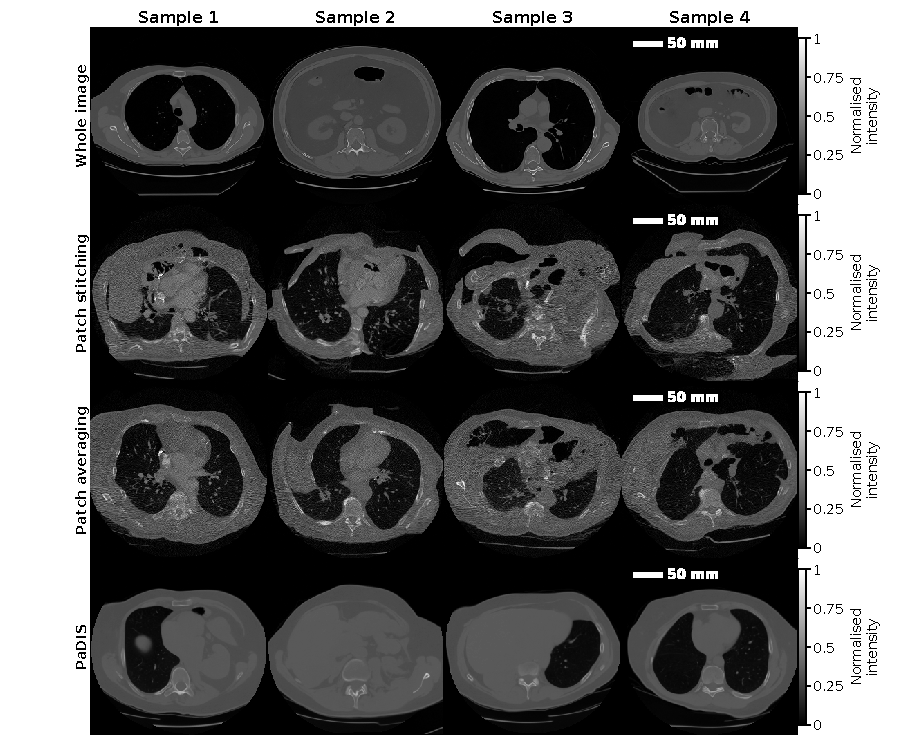
\includegraphics[width=\textwidth]{figure4_generation.pdf}
\caption{[Caption for Figure 4 generation results.]}
\label{fig:results-generation}
\end{figure}
\clearpage

\begin{figure}[p]
\centering
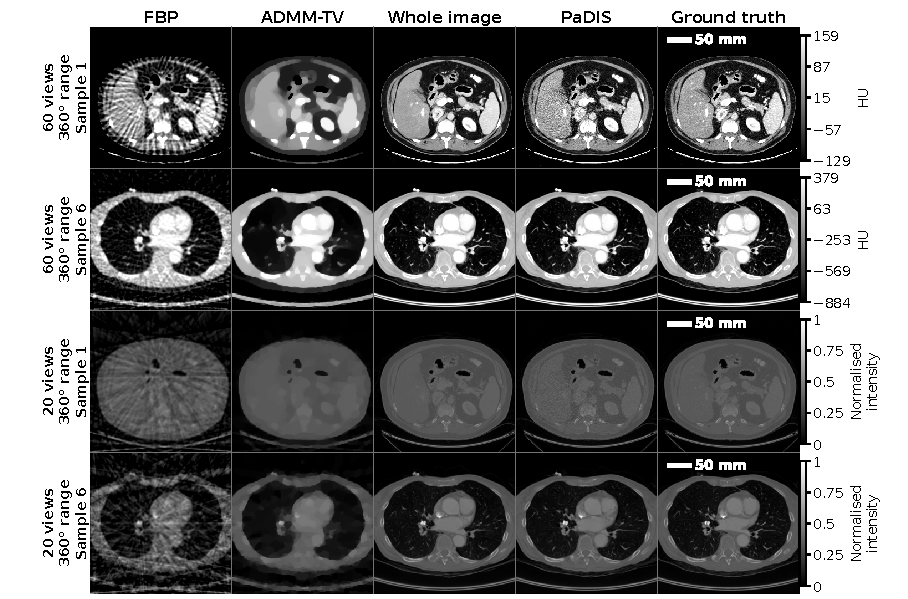
\includegraphics[width=\textwidth]{figure5_ct_reconstruction.pdf}
\caption{[Caption for Figure 5 CT reconstruction results.]}
\label{fig:results-ct-reconstruction}
\end{figure}
\clearpage

\begin{figure}[p]
\centering
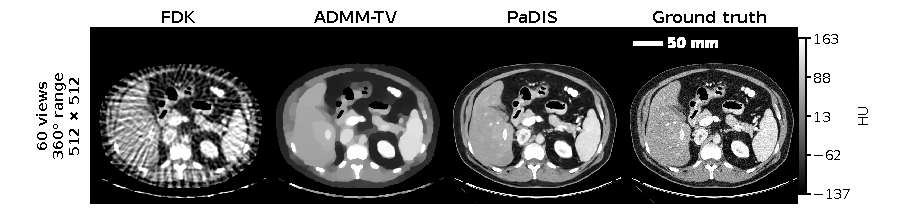
\includegraphics[width=\textwidth]{figure8_512_ct.pdf}
\caption{[Caption for Figure 8, 512 CT results.]}
\label{fig:results-512-ct}
\end{figure}
\clearpage

\begin{figure}[p]
\centering
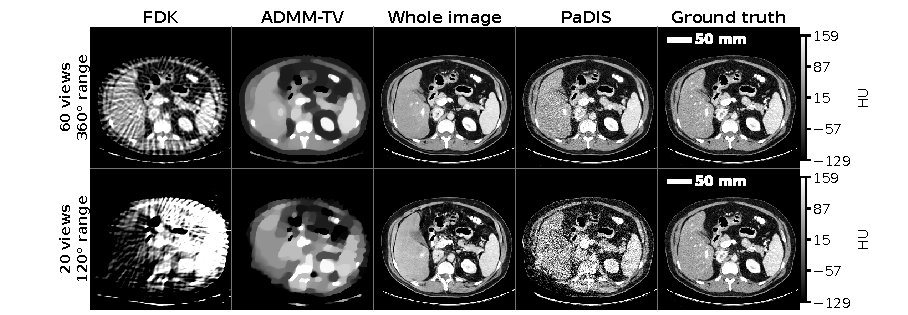
\includegraphics[width=\textwidth]{figureA10_extra_ct.pdf}
\caption{[Caption for Figure A10 additional CT results.]}
\label{fig:results-extra-ct}
\end{figure}
\clearpage

\begin{figure}[p]
\centering
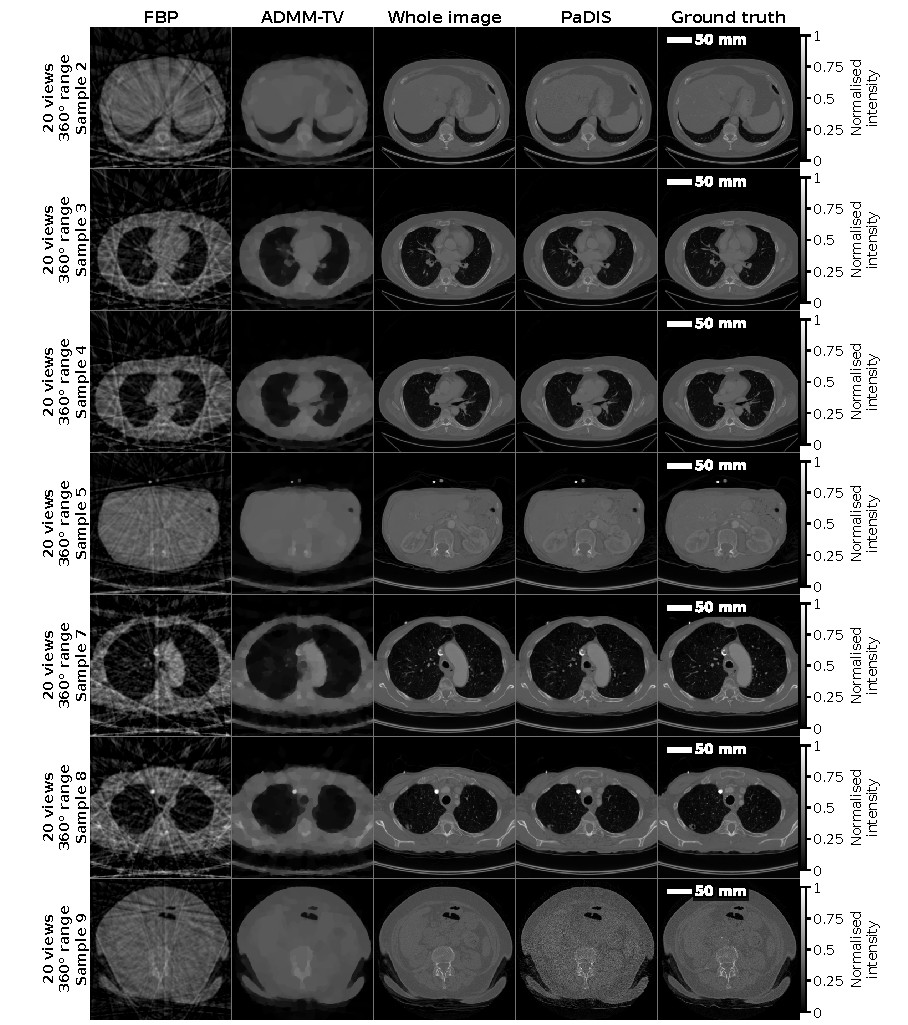
\includegraphics[width=\textwidth]{figureA1_ct20_additional.pdf}
\caption{[Caption for Figure A1, 20-view additional results.]}
\label{fig:results-ct20-additional}
\end{figure}
\clearpage

\begin{figure}[p]
\centering
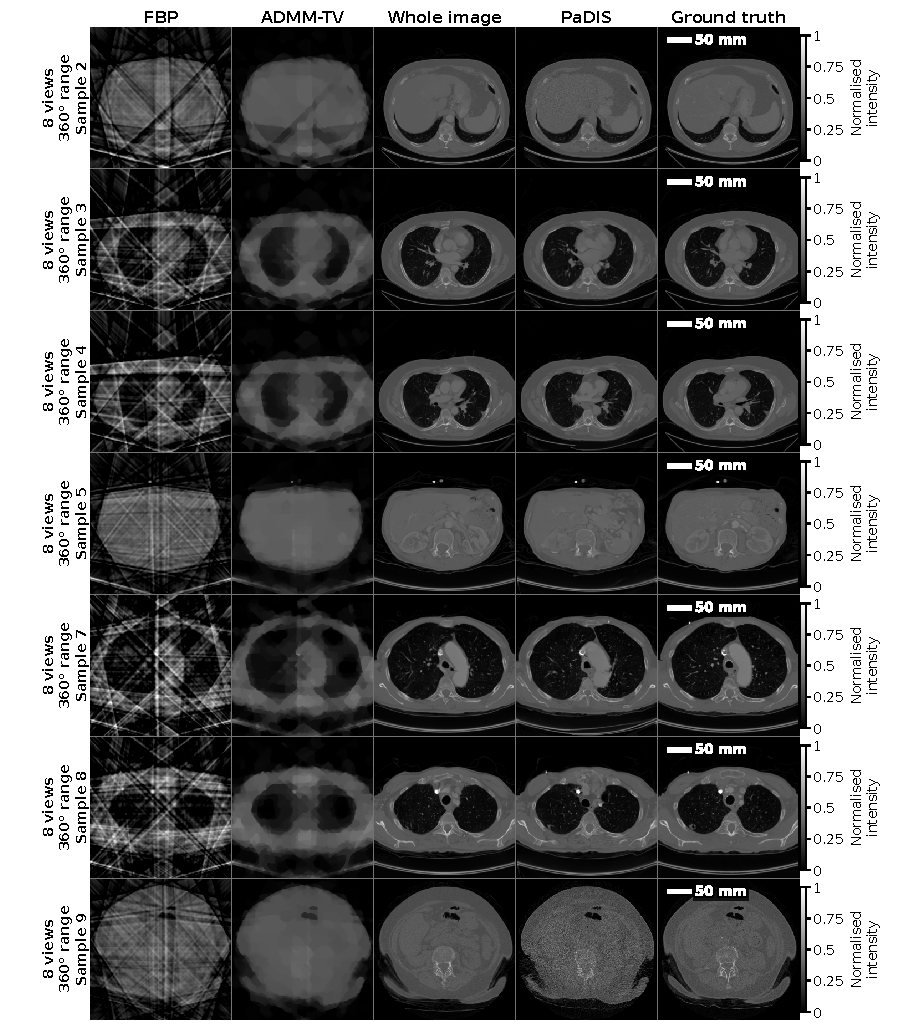
\includegraphics[width=\textwidth]{figureA2_ct8_additional.pdf}
\caption{[Caption for Figure A2, 8-view additional results.]}
\label{fig:results-ct8-additional}
\end{figure}
\clearpage

\begin{figure}[p]
\centering
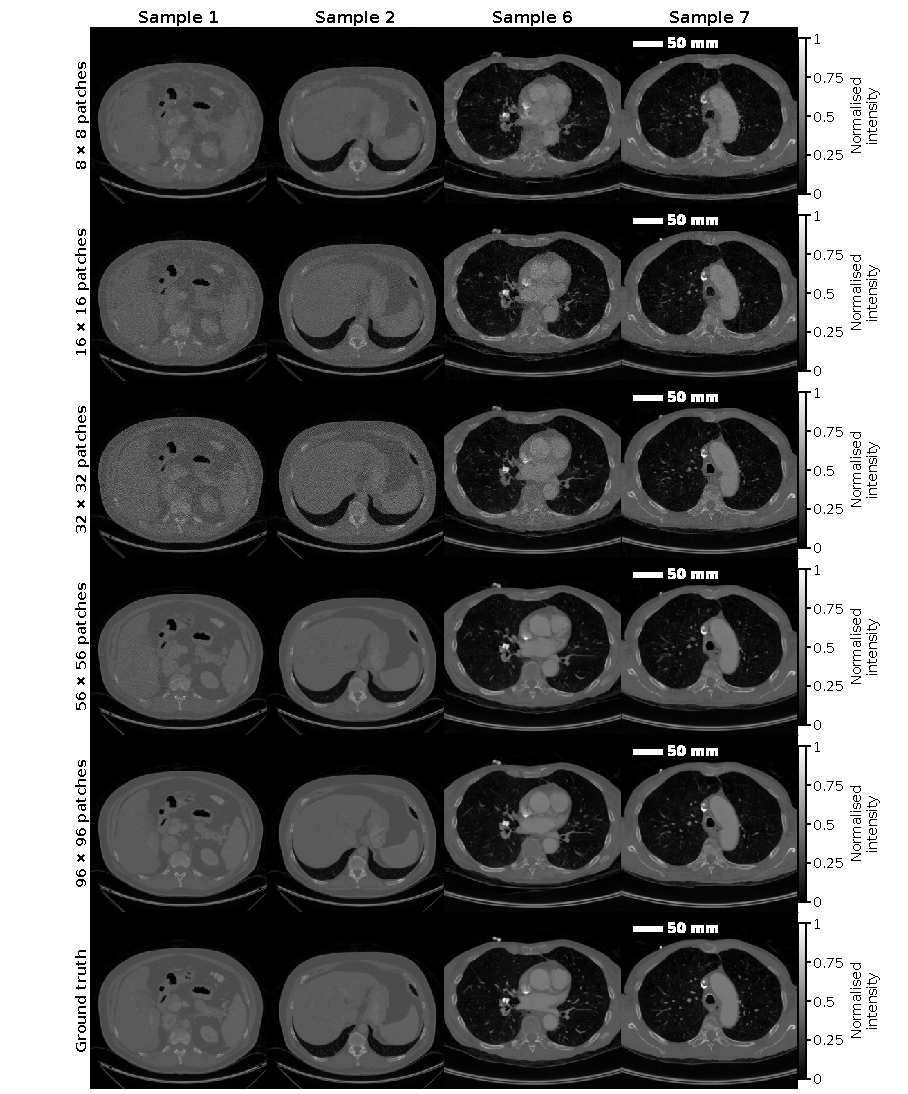
\includegraphics[width=\textwidth]{figureA5_patch_size.pdf}
\caption{[Caption for Figure A5 patch-size ablation.]}
\label{fig:results-patch-size}
\end{figure}
\clearpage

\begin{figure}[p]
\centering
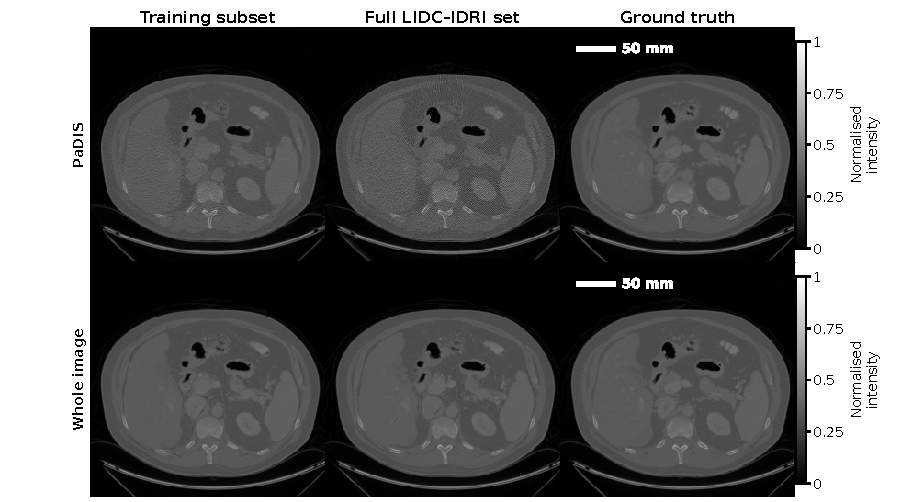
\includegraphics[width=\textwidth]{figureA6_dataset_size.pdf}
\caption{[Caption for Figure A6 dataset-size ablation.]}
\label{fig:results-dataset-size}
\end{figure}
\clearpage

\begin{figure}[p]
\centering
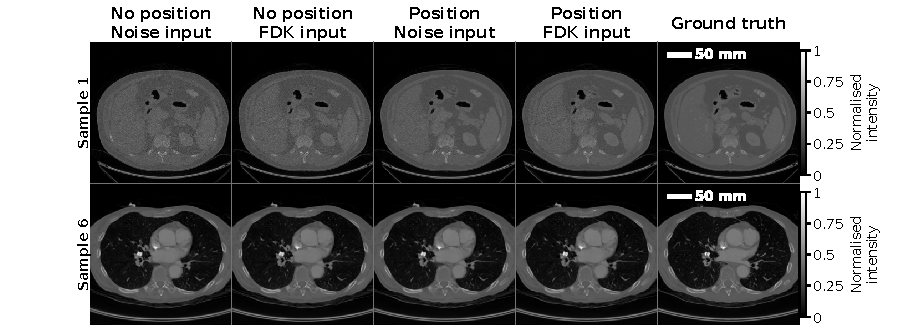
\includegraphics[width=\textwidth]{figureA7_position_encoding.pdf}
\caption{[Caption for Figure A7 position-encoding ablation.]}
\label{fig:results-position-encoding}
\end{figure}
\clearpage

\begin{figure}[p]
\centering
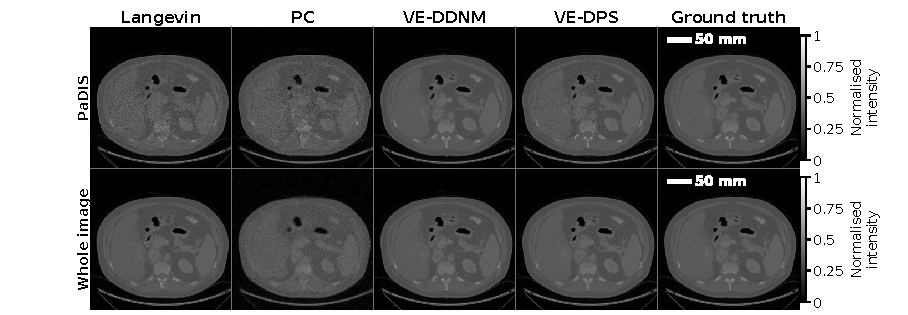
\includegraphics[width=\textwidth]{figureA8_sampling_methods.pdf}
\caption{[Caption for Figure A8 sampling-method comparison.]}
\label{fig:results-sampling-methods}
\end{figure}
\clearpage

%!TEX root = ../thesis.tex
\ifpdf
    \graphicspath{{Sections/5_discussion_figs/Raster/}{Sections/5_discussion_figs/PDF/}{Sections/5_discussion_figs/}}
\else
    \graphicspath{{Sections/5_discussion_figs/Vector/}{Sections/5_discussion_figs/}}
\fi

\chapter{Discussion}
\label{sec:discussion}

\section{Comparison with Hu et al.}

We retained the training and patch-score construction methods of Hu et al. \cite{hu_learning_2024} while moving from AAPM parallel-beam to LIDC-IDRI fan-beam data, allowing us to test the transfer of these methods across datasets and operators.

\subsection{Findings that Transferred}

Hu et al. reported PaDIS-VE-DPS PSNRs of $33.57\,\mathrm{dB}$ at 20 views and $29.48\,\mathrm{dB}$ at 8 views \cite{hu_learning_2024}. Our Paper-Faithful track reached $32.71$ and $27.15\,\mathrm{dB}$. Despite changed data and geometry, the 20-view result is within $0.86\,\mathrm{dB}$, and the 8-view result substantially improves on FDK and CP-TV. PaDIS also generated coherent whole CT slices from patches, whereas fixed stitching and averaging produced less credible anatomies, supporting use of randomly shifted patches.

At $512\times512$, LION-Physical PaDIS-VE-DPS obtained $40.08\,\mathrm{dB}$ PSNR and $0.960$ SSIM, significantly outperforming CP-TV and FDK, and supporting the high-resolution motivation \cite{hu_learning_2024}. PaDIS therefore remains useful where whole-image memory is prohibitive.

\subsection{Findings that Did Not Transfer}

We did not reproduce the claim that PaDIS consistently outperforms whole-image diffusion \cite{hu_learning_2024}. In the Paper-Faithful track, whole-image VE-DPS exceeded PaDIS-VE-DPS by $1.26\,\mathrm{dB}$ at 20 views and $1.95\,\mathrm{dB}$ at 8 views. The LION-Physical comparison showed the same reversal, also visible in \autoref{fig:results-ct20-additional} and \autoref{fig:results-ct8-additional}.

The whole-image prior was not, however, uniformly stronger. Validation-selected LION-Physical PaDIS-VE-DDNM achieved the best 20- and 60-view PSNRs and exceeded its whole-image counterpart by $2.30\,\mathrm{dB}$ at 20 views. Langevin and VE-DPS favoured the whole-image prior, while predictor-corrector rankings depended on the metric. These comparisons do not isolate architecture because settings were validation-selected per prior and sampler, but show that PaDIS performance depends on how its patch score is used.

\subsection{Ablation Findings}

We repeated Hu et al.'s patch-size, training-set-size and positional-encoding ablations \cite{hu_learning_2024} on LIDC-IDRI. The initialisation and schedule comparisons instead address paper--code differences.

Smaller patches gave no consistent benefit. The $96\times96$ model nearly matched whole-image VE-DPS, while the default $56\times56$ model was $1.43\,\mathrm{dB}$ lower. Non-monotonic improvement at $8\times8$ suggests that receptive field, optimisation, patch count and partition geometry all contribute. \autoref{tab:patch-size} and \autoref{fig:results-patch-size} favour global context when memory permits, although non-default models inherited the $P=56$ inference setting and may not be optimal. PaDIS's clearest advantage is therefore feasibility rather than quality from very small patches. Using all processed LIDC-IDRI slices was also not seen to improve PaDIS-VE-DPS under fixed within-prior training time.

Removing position channels reduced PSNR by only $0.3$ to $0.4\,\mathrm{dB}$, in contrast to the failure reported by Hu et al. \cite{hu_learning_2024}. The CT measurements and repeated data-consistency updates appear to provide enough global information to locate local anatomy. This finding remains conditional on the shared inference setting and does not establish that positional channels are unnecessary for unconditional generation, where spatial context cannot be established by measurement-consistency. Similarly, FDK and Gaussian initialisation converged to almost identical results after 1000 model evaluations. The geometric noise schedule had a larger effect, improving PSNR by about $1.3\,\mathrm{dB}$ relative to the original repo EDM-style default.

\subsection{Original PaDIS Specification and Implementation}
\label{sec:discussion-reproducibility}

We treated the released code as part of the specification of the original PaDIS work rather than as a separate implementation \cite{hu_learning_2024,hu_jasonhu4padis_2026-1}. Together, the paper and code leave choices ambiguous. The variable-size U-Net is attributed to different references, while the number of sampled patches, validation split, checkpoint rule and selection of 25 test slices are not reported. View and detector counts are given without the physical field of view, detector spacing or complete angular conventions needed to define $A$. The released 180-view fan-beam configuration also spans only $180^\circ$, which is not explicit in the main description. Fine-tuning is reported without the search or selection protocol. Inconsistencies include their Table 1 not always bolding the best SSIM and their Table 7 describing a dataset-size analysis despite comparing samplers.

The implementations in the corresponding released repository resolve some details but differ from the algorithms in the original PaDIS paper \cite{hu_learning_2024,hu_jasonhu4padis_2026-1}. The main VE-DPS path starts from filtered back-projection rather than the Gaussian state in Algorithm 1 of the paper, differentiates the residual norm rather than its square and defaults to an EDM-style schedule. The predictor--corrector path evaluates the corrector denoiser at the current level, $\sigma_k$, but divides the denoising residual by $\sigma_{k+1}^2$ and reuses the patch layout drawn for the predictor. The paper reports 1000 neural function evaluations (NFEs) for all diffusion experiments, whereas the released CT command uses 100 noise levels. Their VE-DPS, Langevin, and DDNM implementations then retain 1000 evaluations through 10 updates per level. Their Predictor--corrector implementation instead makes two evaluations between adjacent levels, totalling 198. The repository also advertises a CT checkpoint, but the Google Drive link returns a file does not exist error. Several hidden APIs also had to be re-integrated before the comparison methods in the repository could be run. As demonstrated in \autoref{tab:main-quality} and \autoref{tab:position}, these paper--code differences do materially change reconstruction.



\section{Extensions to the Original Work}

Paper-Faithful and Repo-Faithful represent two readings of the combined specification. LION-Physical is our extension and replaces geometry-specific calibration with an operator-derived scale. Its results assess transfer and stabilisation rather than direct reproduction of Hu et al.'s algorithms.

\subsection{Operator-Normalised Data Consistency}

The LION-Physical VE-DPS rows reached relative sinogram residuals near $10^{-3}$, over an order of magnitude below many Paper-Faithful and Repo-Faithful results. Diffusion models can otherwise produce plausible images that are not well supported by the measurements. In the limited-angle experiment, whole-image VE-DPS gave the best PSNR and SSIM, while PaDIS-VE-DPS gave the smallest residual. There is therefore a trade-off between similarity to the held-out target and strict agreement with the measured data.

The Repo-Faithful fan-beam updates required calibrated gradient scales of $0.0405$ and $0.1022$. Replacing them with operator normalisation based on $\lVert F\rVert_2^2$ still gave high-quality results across the angular settings. These constants therefore correct for a particular implementation rather than defining PaDIS itself. Operator normalisation is more reproducible because it remains meaningful when the geometry changes.

\subsection{Fixed Patch Assembly}

Fixed averaging obtained the highest reported SSIM and lowest MAE in parts of \autoref{tab:main-quality}, but these rows contain only four images and have wide uncertainty. Its unconditional samples also lacked credible global anatomy. These results show that overlap handling can suppress seams but do not establish an improvement over random PaDIS partitions.

\section{Limitations and Future Work}

As in the original CT experiments of Hu et al. \cite{hu_learning_2024}, our sinograms omit photon noise, scatter, beam hardening and motion. We therefore investigate angular undersampling rather than realistic low-dose CT. The experiments are two-dimensional, use one dataset and one training run per model, and evaluate 25 slices rather than independent scans. The fixed-overlap and native-resolution rows use four images. Bootstrap intervals measure variation across slices rather than retraining uncertainty. Some high-view methods inherit 20-view tuning, and we did not tune the patch-size and no-position rows per model. PSNR, SSIM and MAE also cannot determine whether a nodule was preserved or hallucinated.

Future work should add calibrated photon noise and task-level evaluation of clinically relevant features. Equal-epoch, multi-seed training would separate dataset size from optimisation time. Averaging scores over several partitions, or a lower-variance deterministic estimator, may help with accelerated samplers. External datasets and expert assessment are required before making clinical claims.

Overall, we reproduce the ability of PaDIS to assemble coherent, high-quality reconstructions from patch scores, including at native resolution. We do not reproduce universal superiority over whole-image diffusion. Instead, our results show where PaDIS is useful, which implementation choices change its ranking and how operator-derived scaling improves transfer between CT geometries.

%!TEX root = ../thesis.tex
\ifpdf
    \graphicspath{{Sections/6_conclusions_figs/Raster/}{Sections/6_conclusions_figs/PDF/}{Sections/6_conclusions_figs/}}
\else
    \graphicspath{{Sections/6_conclusions_figs/Vector/}{Sections/6_conclusions_figs/}}
\fi

\chapter{Conclusion}
\label{sec:conclusion}

In this work, we reproduced PaDIS in LION and showed that patch-trained diffusion priors support accurate, data-consistent fan-beam CT reconstruction at up to $512\times512$, but not that PaDIS consistently outperforms whole-image diffusion. Under VE-DPS, we found the opposite ranking, while PaDIS-VE-DDNM was strongest at 20 and 60 views. Patch size and sampler choice mattered more than positional encoding or the number of training slices under fixed compute. PaDIS is therefore a memory-scalable high-resolution prior whose value depends on the reconstruction method, while our LION-Physical extension with operator-derived scaling improves data consistency across CT geometries. Underspecificaitons in the original PaDIS are also highlighted, demonstrating the importantce of complete geometry, training, tuning and executable algorithm specifications in inverse-problem research.

%\include{Chapter4/chapter4}
%\include{Chapter5/chapter5}
%\include{Chapter6/chapter6}
%\include{Chapter7/chapter7}



% ********************************** Back Matter *******************************
% Backmatter should be commented out, if you are using appendices after References
%\backmatter

% ********************************** Bibliography ******************************
\begin{spacing}{0.9}

% To use the conventional natbib style referencing
% Bibliography style previews: http://nodonn.tipido.net/bibstyle.php
% Reference styles: http://sites.stat.psu.edu/~surajit/present/bib.htm

\bibliographystyle{unsrt} % Number references in order of first appearance
%\bibliographystyle{apalike}
%\bibliographystyle{plainnat} % use this to have URLs listed in References
\cleardoublepage
\phantomsection
\begingroup
\raggedright
\bibliography{References/references} % Path to your References.bib file
\endgroup


% If you would like to use BibLaTeX for your references, pass `custombib' as
% an option in the document class. The location of 'reference.bib' should be
% specified in the preamble.tex file in the custombib section.
% Comment out the lines related to natbib above and uncomment the following line.

%\printbibliography[heading=bibintoc, title={References}]


\end{spacing}

% ********************************** Appendices ********************************

\begin{appendices} % Using appendices environment for more functunality

\wordcountexclude{Sections/7_appendix_llms}
\ifpdf
    \graphicspath{{Sections/4_results_figs/Raster/}{Sections/4_results_figs/PDF/}{Sections/4_results_figs/}}
\else
    \graphicspath{{Sections/4_results_figs/Vector/}{Sections/4_results_figs/}}
\fi

\chapter{Additional Figures}
\label{chap:additional-figures}

This appendix contains the extended 20- and 8-view examples and the full patch-size panel. Dataset-size, position and sampler figures are placed with their analyses in the Results section.

\begin{figure}[htbp]
\centering
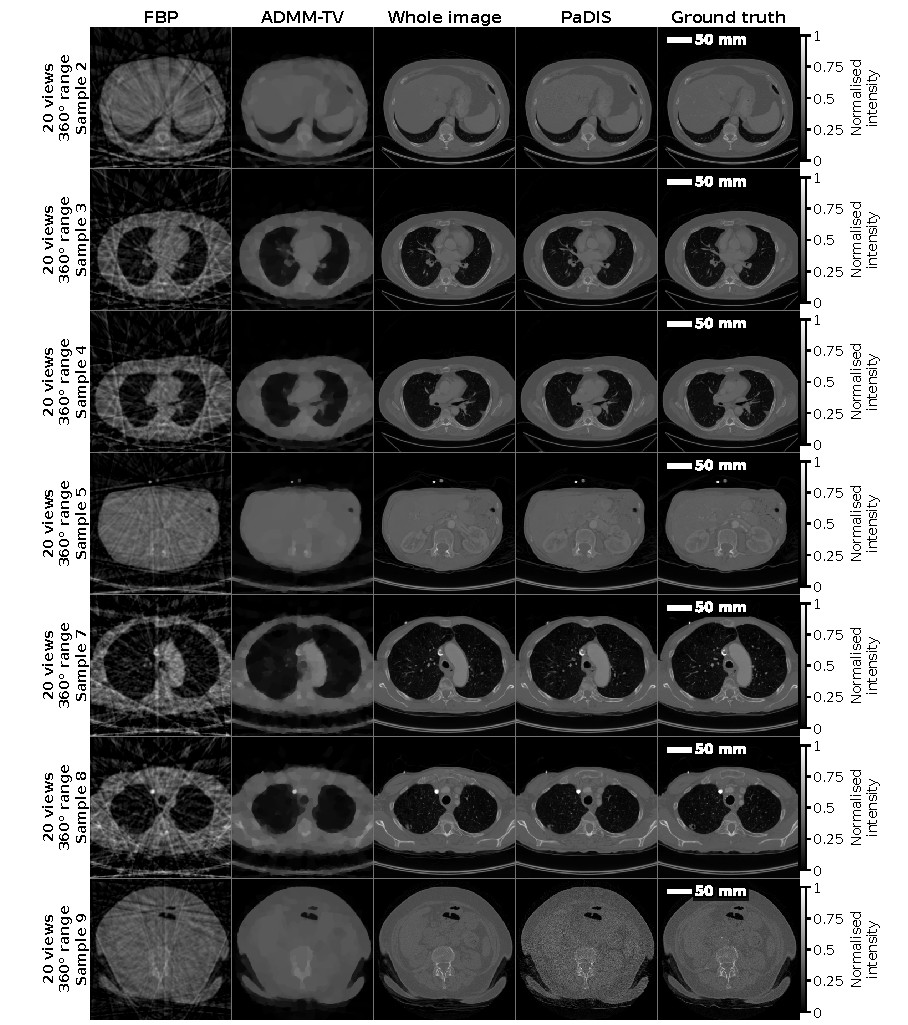
\includegraphics[width=1\textwidth]{figureA1_ct20_additional.pdf}
\caption[Additional 20-view examples.]{Additional 20-view, $360^\circ$ fan-beam examples in NI. Rows are test slices and columns compare FDK, CP, whole-image VE-DPS, PaDIS-VE-DPS and ground truth.}
\label{fig:results-ct20-additional}
\end{figure}

\begin{figure}[htbp]
\centering
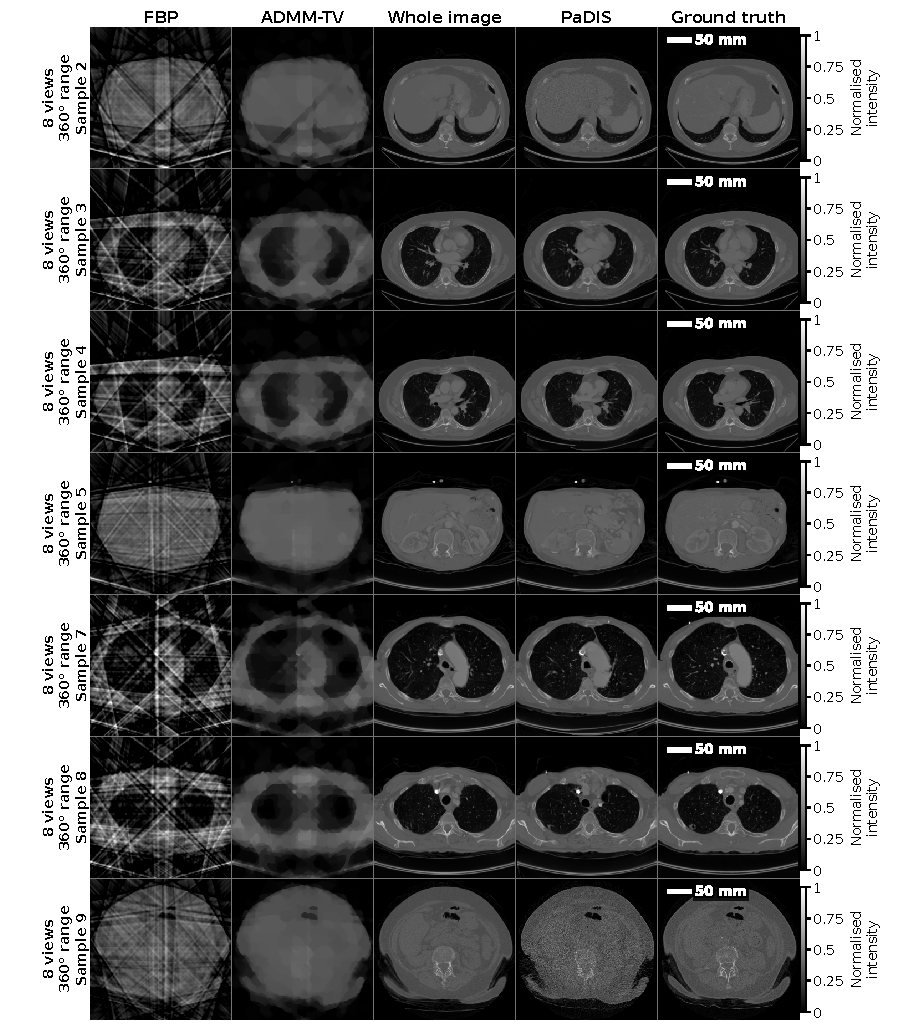
\includegraphics[width=1\textwidth]{figureA2_ct8_additional.pdf}
\caption[Additional 8-view examples.]{Additional 8-view, $360^\circ$ fan-beam examples in NI. Rows are test slices and columns compare FDK, CP, whole-image VE-DPS, PaDIS-VE-DPS and ground truth.}
\label{fig:results-ct8-additional}
\end{figure}

\begin{figure}[htbp]
\centering
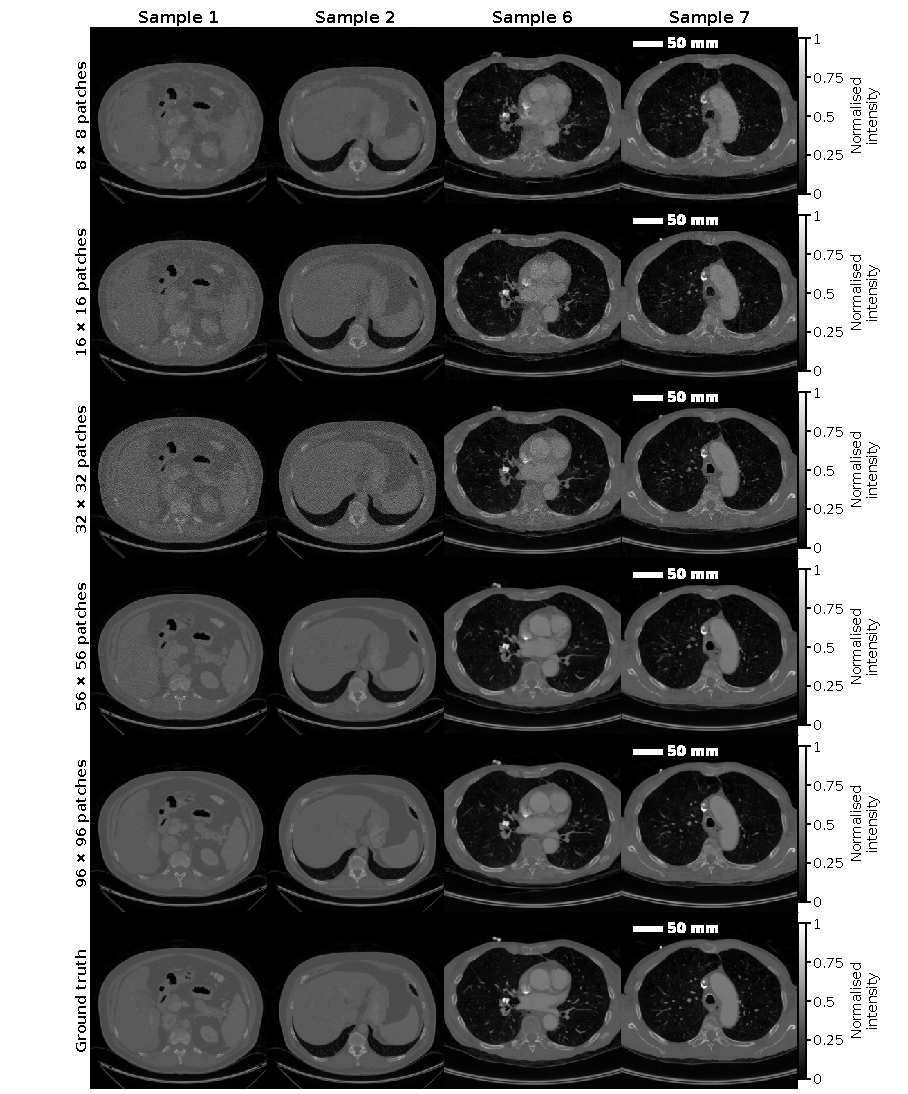
\includegraphics[width=1\textwidth]{figureA5_patch_size.pdf}
\caption[Patch-size reconstruction examples.]{PaDIS-VE-DPS reconstructions from the patch-size ablation in NI. Rows show the maximum training patch size and ground truth. Columns are four test slices. The non-default models inherit the $P=56$ inference setting rather than being tuned separately.}
\label{fig:results-patch-size}
\end{figure}

\chapter{Indicative Reconstruction Times}
\label{app:runtime}

Possible GPU sharing makes timings approximate. PaDIS-DPS took about two minutes per slice, $24\%$ below whole-image VE-DPS. Fixed patch methods took about $24$ minutes.

\begin{table}[htbp]
\centering
\caption[Logged reconstruction time per slice.]{Mean 20-view time per slice from pipeline logs.}\label{tab:runtime}
\small
\begin{tabular}{llr}
\toprule[1.1pt]
\multicolumn{1}{l}{\bfseries Implementation} & \multicolumn{1}{l}{\bfseries Reconstruction method} & \multicolumn{1}{r}{\bfseries Mean time per slice} \\
\midrule
\textbf{LION-Physical} & Baseline & \textbf{4.71 s} \\
 & CP & 8.13 s \\
 & Predictor--corrector & 14.11 s \\
 & PnP--ADMM & 26.63 s \\
 & Langevin & 51.49 s \\
 & VE--DDNM & 62.08 s \\
 & PaDIS--DPS & 118.85 s \\
 & VE--DPS (Whole-Image) & 156.44 s \\
 & Patch stitch & 1,450.73 s (24.18 min) \\
 & Patch average & 1,468.76 s (24.48 min) \\
\midrule
\textbf{Paper-Faithful} & Predictor--corrector & 14.16 s \\
 & Langevin & 56.42 s \\
 & VE--DDNM & 61.34 s \\
 & PaDIS--DPS & 120.45 s \\
 & VE--DPS (Whole-Image) & 156.89 s \\
\midrule
\textbf{Repo-Faithful} & Predictor--corrector & 14.02 s \\
 & Langevin & 56.55 s \\
 & VE--DDNM & 58.54 s \\
 & PaDIS--DPS & 119.22 s \\
 & Patch stitch & 1,461.08 s (24.35 min) \\
 & Patch average & 1,468.75 s (24.48 min) \\
\bottomrule[1.1pt]
\end{tabular}
\end{table}

%!TEX root = ../thesis.tex
\chapter{Diffusion Training Exposure}
\label{app:training-exposure}

\begin{table}[htbp]
\centering
\caption[Diffusion training exposure.]{Final Weights \& Biases training counters. Whole-image rows count complete images, while PaDIS rows count sampled patches. Model labels link to their runs.}
\label{tab:training-exposure}
\small
\begin{tabular}{lr}
\toprule[1.1pt]
\textbf{Model} & \textbf{Samples seen} \\
\midrule
\href{https://wandb.ai/tjh200-university-of-cambridge/PaDIS-Reproduction/runs/xq69oaui}{Whole image, default data} & 1,239,000 \\
\href{https://wandb.ai/tjh200-university-of-cambridge/PaDIS-Reproduction/runs/9e3903d7}{Whole image, all data} & 1,224,536 \\
\midrule
\href{https://wandb.ai/tjh200-university-of-cambridge/PaDIS-Reproduction/runs/3r8yjo1x}{PaDIS, default} & 30,576,000 \\
\href{https://wandb.ai/tjh200-university-of-cambridge/PaDIS-Reproduction/runs/vd4zu3h2}{PaDIS, all data} & 30,293,504 \\
\href{https://wandb.ai/tjh200-university-of-cambridge/PaDIS-Reproduction/runs/k3ewkq7y}{PaDIS, $512\times512$} & 19,828,224 \\
\href{https://wandb.ai/tjh200-university-of-cambridge/PaDIS-Reproduction/runs/zgivu4ud}{PaDIS, $P=8$} & 100,539,904 \\
\href{https://wandb.ai/tjh200-university-of-cambridge/PaDIS-Reproduction/runs/uaasmrt6}{PaDIS, $P=16$} & 107,610,624 \\
\href{https://wandb.ai/tjh200-university-of-cambridge/PaDIS-Reproduction/runs/88014kal}{PaDIS, $P=32$} & 78,504,576 \\
\href{https://wandb.ai/tjh200-university-of-cambridge/PaDIS-Reproduction/runs/e24q8o1e}{PaDIS, $P=96$} & 9,906,944 \\
\href{https://wandb.ai/tjh200-university-of-cambridge/PaDIS-Reproduction/runs/aqh1bipv}{PaDIS, no position channels} & 30,199,808 \\
\bottomrule[1.1pt]
\end{tabular}
\end{table}


% If you have an "Auto-generation usage" appendix that must be excluded from the
% policy-required report word count, wrap it with the helper macro:
%   \wordcountexclude{AppendixX/auto-generation-tools}

\end{appendices}

% *************************************** Index ********************************
% No index is present, so do not emit an empty index page.
% \printthesisindex

\end{document}
